\newcommand{\econtexRoot}{..}
% The \commands below are required to allow sharing of the same base code via Github between TeXLive on a local machine and ShareLaTeX.  This is an ugly solution to the requirement that custom LaTeX packages be accessible, and that ShareLaTeX seems to ignore symbolic links (even if they are relative links to valid locations)
\providecommand{\econtex}{./texmf-local/tex/latex/econtex}
\providecommand{\econtexSetup}{./texmf-local/tex/latex/econtexSetup}
\providecommand{\econtexShortcuts}{./texmf-local/tex/latex/econtexShortcuts}
\providecommand{\econtexBibMake}{./texmf-local/tex/latex/econtexBibMake}
\providecommand{\econtexBibStyle}{./texmf-local/bibtex/bst/econtex}
\providecommand{\notes}{./texmf-local/tex/latex/handout}
\providecommand{\handoutSetup}{./texmf-local/tex/latex/handoutSetup}
\providecommand{\handoutShortcuts}{./texmf-local/tex/latex/handoutShortcuts}
\providecommand{\handoutBibMake}{./texmf-local/tex/latex/handoutBibMake}
\providecommand{\handoutBibStyle}{./texmf-local/bibtex/bst/handout}

  
\documentclass[titlepage]{\econtex}\newcommand{\texname}{cjSOE}

\usepackage{\econtexSetup}\usepackage{\econtexShortcuts}\usepackage{\econtexShortcuts}
\usepackage{\econtexRoot/cjSOE}
\usepackage{subfiles}

\usepackage{layouts,rotating,psfrag,amssymb}

\renewcommand{\GDPLev}{\ensuremath{\pmb{Y}}}
\renewcommand{\gdpLev}{\ensuremath{\pmb{y}}}
\renewcommand{\ptyLev}{\ensuremath{z}}


\opt{JournalFormatting}{\renewcommand{\footnote}{\endnote}}

\hypersetup{pdfauthor={Christopher Carroll <ccarroll@jhu.edu>, Olivier Jeanne <ojeanne@jhu.edu>},
            pdfsubject={A Tractable Model of Precautionary Reserves, Net Foreign Assets, or Sovereign Wealth Funds},
            pdfkeywords={Consumption, Saving, Net Foreign Assets, Foreign Reserves},
            pdfproducer = {LaTeX with hyperref and thumbpdf},
            pdfcreator = {ps2pdf, pdfwrite}
            }

\begin{document}\bibliographystyle{econtex}

\opt{JournalFormatting}{\doublespacing}

\begin{verbatimwrite}{\jobname.title}
A Tractable Model of Precautionary Reserves, Net Foreign Assets, or Sovereign Wealth Funds
\end{verbatimwrite}

\title{\Large A Tractable Model of Precautionary Reserves, \\ Net Foreign Assets, or Sovereign Wealth Funds \\ {\phantom{\tiny ~}} }

\medskip\medskip

\ifdvi    % CDCPrivate
  \large  % CDCPrivate
\fi       % CDCPrivate

\newcommand{\forceSpace}{\ifdvi {\tiny .} \fi} % For html version, kludge to force a space to be inserted
\author{
{Christopher D. Carroll\tiny{~}}\num \\ \forceSpace 
\and 
{Olivier Jeanne\tiny{~}}\num \\ \forceSpace
}



\keywords{\noindent Buffer Stock Saving, Net Foreign Assets, Sovereign Wealth Funds, Foreign Exchange Reserves, Small Open Economy}
\jelclass{C61}

%\maketitle
\maketitleWithForcedDate{February 2019} %\boldred{Preliminary Draft}}

\begin{abstract}
  \opt{JournalFormatting}{\doublespacing} We model the motives for residents of a country to hold foreign
  assets, including the precautionary motive that has been omitted
  from much previous literature as intractable.  Our model captures
  the principal insights from the existing literature on
  the precautionary motive with a novel and convenient formula for the
  economy's target asset ratio.  The target is the value of assets
  that balances growth, impatience, prudence, risk, intertemporal
  substitution, and the rate of return.  We use the model to shed
  light on two topical questions: ``Upstream'' flows of capital from
  developing to advanced countries, and the long-run impact of
  resorbtion of global financial imbalances.
\end{abstract}

\begin{small}
\parbox{\textwidth}{
\begin{center}
\begin{tabbing}
\texttt{Archive:~} \= \= \url{http://econ.jhu.edu/people/ccarroll/papers/cjSOE.zip} \kill \\  % This line establishes the locations of the tabs, but is not printed
\texttt{~~~~PDF:~}\> \> \url{http://econ.jhu.edu/people/ccarroll/papers/cjSOE.pdf} \\
\texttt{~Slides:~}\> \> \url{http://econ.jhu.edu/people/ccarroll/papers/cjSOE-Slides.pdf} \\
\texttt{~~~~Web:~} \> \> \url{http://econ.jhu.edu/people/ccarroll/papers/cjSOE/}    \\
\texttt{~~~Repo:~} \> \> \url{https://github.com/llorracc/cjSOE} \\
%\texttt{~~~Code:~} \> \> \url{http://econ.jhu.edu/people/ccarroll/code/Tractable.zip} \\
\texttt{~~~~~~~~~} \> \> {\it (Contains code solving this paper's model (and related models))}
\end{tabbing}
\end{center}
}
\end{small}

\begin{authorsinfo}
\name{Carroll: \href{mailto:ccarroll@jhu.edu}{\texttt{ccarroll@jhu.edu}}, Department of Economics, 440 Mergenthaler Hall,
Johns Hopkins University, Baltimore, MD 21218, \url{http://econ.jhu.edu/people/ccarroll/}, and National Bureau of Economic Research.}
\\
\name{Jeanne: \href{mailto:ojeanne@jhu.edu}{\texttt{ojeanne@jhu.edu}}, Department of Economics, 440 Mergenthaler Hall,
Johns Hopkins University, Baltimore, MD 21218, \url{http://econ.jhu.edu/people/jeanne/}, and National Bureau of Economic Research.}
\end{authorsinfo}

\thanks{We thank Romain Ranci\`ere for an insightful discussion of the
  paper at the 2009 ASSA meetings, and seminar participants at George
  Washington University, the Federal Reserve Bank of San Francisco,
  and the Bank of Canada for their comments, Patrick Toche for
  comments, and Matthew White and Jiaxiong Yao for excellent research assistance.  This draft corrects some minor errors in the previous draft, and updates the solution code to be much faster.}

\titlepagefinish
\setcounter{page}{1}

\section{Introduction} 

The remarkable accumulation of foreign reserves in emerging
economies has captured the attention of academics, policymakers, and
financial markets, partly because reserve accumulation seems to have
played a role in the development of global financial imbalances.  A
distinct (but probably related) puzzle is that national saving rates
of fast-growing emerging economies have been rising over
time,\footnote{For evidence of causality from growth to saving, see
  \cite{carroll&weil:crcs}; \cite{lss:whatdrives}; \cite{aps:sgi};
  \cite{hprGrowth}; \cite{gourinchasJeannePuzzle}.} leading to
surprising ``upstream'' flows of capital from developing to rich
countries.  The corresponding accumulation of foreign assets in
``sovereign wealth funds'' has also attracted scrutiny as those
funds have emerged as prominent actors in global capital markets.

A popular interpretation of all these trends is that they
reflect precautionary saving against the risks associated with
economic globalization.\footnote{``The East Asian countries that constitute the class of '97---the countries that learned the lessons
of instability the hard way in the crises that began that year---have boosted their reserves in part because they want to make sure that they won't need
to borrow from the IMF again. Others, who saw their neighbors suffer, came to the same conclusion---it is imperative to have enough reserves
to withstand the worst of the world's economic vicissitudes.'' (Stiglitz, 2006, p. 248)}

Such an interpretation raises several questions. What are the main
determinants of the demand for external assets?  What are the welfare
benefits of international integration, if it leads developing
countries to export rather than import capital?  How persistent will
the increase in developing countries' demand for foreign assets
prove to be?  How does the precautionary motive for asset
accumulation interact with other, better-understood motives?

This paper introduces a tractable model that can be used to analyze
these questions (and others). Our model is a small-open-macroeconomy
version of the model of individual precautionary saving developed
by~\cite{carrollTractable}, based on~\cite{toche:urisk}. With it, 
we characterize the dynamics of foreign asset accumulation
using phase diagrams that should be readily understandable to anyone
familiar with the benchmark Ramsey model of economic growth, and we 
derive closed-form expressions that relate the target level of net
foreign assets to fundamental determinants like the degree of risk,
the time preference rate, and expected productivity growth.  The
model's structure is simple enough to permit straightforward
calculations of welfare-equivalent tradeoffs between growth, social
insurance generosity, and risk.

We then present two applications of our framework. 

First, we look at what the model says about the puzzling relation
between economic growth and international capital flows (especially
the fact that fast-growing developing countries tend to export
capital).  Several recent papers (e.g., \cite{clpChinaSaving} and
\cite{wenChinaSaving}) argue in particular that the rise in China's
saving rate reflects precautionary motives.  We show that merely
adding precautionary saving to the usual intertemporal optimization
framework does not reverse that model's implication that exogenously
higher growth should cause lower saving.  But the growth-to-saving
puzzle can be explained in our framework if the bargain that countries
make when they embark on a path of rapid development involves not only
a pickup in productivity growth but also an increase in the degree of
idiosyncratic risk borne by individuals (like unemployment spells that
result in substantial lost wages).\footnote{Little relevant empirical
evidence appears to exist for judging the plausibility of this condition;
we hope that our model's clarification of what to look for might stimulate 
the relevant empirical studies.}

Second, we use a two-country version of the model to investigate the
long-term impact on the United States and the rest of the world if the
recent global financial imbalances were to be resorbed by a fall in
non-U.S.\ savings (as some analysts have urged). Our model implies
that a decrease in the desired level of wealth in the rest of the
world has a substantial negative impact on the global capital stock as
well as the U.S.\ (and global) real wage.

A central purpose of the paper is to distill the main insights of the
complex literature that interprets capital flows through the lens of
the precautionary motive. We aim to
improve on an older literature on the `intertemporal approach to the
current account' that simply ignores precautionary behavior by
considering a linear-quadratic formulation of the consumption-saving
problem (see~\cite{orIntertemporal} for a review).\footnote{An exception
is~\cite{goJME}, who look at the implications of precautionary motives
for the current account balance of advanced economies. They use a
model with aggregate income shocks in which the domestic consumer has
constant absolute risk aversion utility (an assumption that makes the
model solvable in closed form but also implies rather special
properties for the dynamics of foreign assets).}

More recently, one strand of the intertemporal literature looks at the
effects of aggregate risk on domestic precautionary wealth. For
example, \cite{dmtMercant} present some estimates of the optimal level
of precautionary wealth accumulated by a small open economy in
response to business cycle volatility, financial globalization, and
the risk of a sudden stop in credit. They conclude that these risks
are plausible explanations of the observed surge in reserves in
emerging market countries.\footnote{In contrast,
  \cite{JeanneBrookings} and \cite{JRreserves} find that it is
  difficult to explain the build-up in emerging markets reserves as
  insurance against the risk of sudden stop.}  \cite{arbatliThesis}
argues that precautionary motives associated with the possibility of
sudden stops can explain the dynamics of the current account in
emerging economy business cycles.  \cite{fogliPerriMod} instead take
the perspective of the U.S.\ and argue that the decrease in its saving
rate can be explained partly by the moderation in the volatility of
its business cycle.

Closer to our paper are the contributions that examine the impact of
idiosyncratic risk on saving behavior. \cite{mqrImbal} model the
determination of capital flows in a closed world in which economies
differ by their level of financial development (market
completeness). They find that international financial integration can
lead to the accumulation of a large level of net and gross liabilities
by the more financially advanced region. \cite{sandri:growthcapflows}
presents a model in which growth acceleration in a developing country
causes a larger increase in saving than in investment because capital
market imperfections induce entrepreneurs not only to self-finance
investment but also to accumulate precautionary wealth outside their
business enterprise.
Another recent contribution is by \cite{paEntrep}, who adapt a
\cite{merton:restat}-\cite{samuelson:portfolio} model of portfolio
choice to a general equilibrium context in which the risky asset, in
each country, is interpreted as reflecting returns to entrepreneurial activity with an
undiversifiable risky component.  They calibrate the degree of
financial development by the magnitude of the undiversifiable
component of entrepreneurial risk.
When a regime change suddenly allows international mobility of the
riskless asset in their model, the result is an immediate large reallocation of risky
capital from the less to the more developed economy.\footnote{See also \cite{Benhima2013} for an application of the \cite{merton:restat}-\cite{samuelson:portfolio} framework to a model on the relationship between growth and the direction of capital flows.}

The recent literature offers several explanations for the accumulation of foreign assets in high-growth emerging market economies that involve financial frictions other than the lack of insurance against income risk.
For example, \cite{cfg:globimbalances} suggest that those flows have been driven by countries' supply of (rather than  demand for) assets. \cite{SongStorenslettenZilibotti11} present a model in which capital flows upstream from a high-growth country because of a friction in the intermediation of domestic saving.
\cite{AguiarAmador11} explain the capital outflows by the accumulation of foreign exchange reserves that are posted as a
  ``bond" to prevent the expropriation of investors.
\cite{CoeurdacierGuibaudJin2015} show that in an open-economy model with overlapping generations, the interaction between growth differentials and household credit constraints can explain the divergence in private saving rates between advanced and emerging economies.
\cite{BachettaBenhima2015} present a model in which firms in a high-growth economy are credit-constrained and need to accumulate funds in order to finance working capital (see also 
\cite{BueraShin2009} for a similar mechanism).  

Also related is recent work by \cite{barroDisasters}, reviving the
proposal of \cite{reitzDisasters} that the equity premium puzzle can
be explained by a fear of rare but catastrophic events.  Our model's
risk is to the consumer's labor income rather than to an investor's
financial returns, but our framework shares the intuition that
precautionary behavior against occasional disasters is powerful even
in periods when the disasters are not observed. 

Several of our analytical results resonate with themes developed quantitatively (or
at least touched upon) in the papers cited above (in particular, the importance of
domestic financial development or social insurance for international
capital flows). The main comparative advantages of our analysis are
three.  First, the insights are reflected in tractable analytical
formulas. The impact of key variables can be analyzed using a simple
diagram or closed-form expressions---although (as usual) analysis of
transitional dynamics requires numerical solution tools (which we
provide).\footnote{\cite{paEntrep} also achieve
  tractability, by building on the Merton-Samuelson model
  of consumption and portfolio choice.  But that model's exclusive
  focus on financial risks (it assumes noncapital income is perfectly
  certain) makes it unusable for many of the questions we address,
  such as the potential role of social insurance in diminishing
  precautionary saving.}  Second, our model of prudent (\cite{kimball:smallandlarge})
intertemporal choice is integrated with a standard neoclassical
treatment of production (Cobb-Douglas with labor augmenting
productivity growth), so that the familiar Ramsey-Cass-Koopmans
framework can be viewed as the perfect-insurance special case of our
model. This allows us analyze the link between economic development
and capital flows in a way that is directly comparable to the
corresponding analysis in the standard model.\footnote{The models of
  \cite{fogliPerriMod} and \cite{mqrImbal} do not incorporate
  growth. The model of \cite{sandri:growthcapflows} has economic
  growth in the transition dynamics toward a long-run steady state
  with no growth. By contrast, our model allows one to look at the
  impact of different long-run productivity growth rates. }
Finally, we do not believe that a model of China's (or Japan's, or Korea's)
high saving can be fully persuasive without explicitly tackling the
relationship of increased saving to rapid economic growth.  The
financial flows from developing to developed countries in
\cite{mqrImbal} are not related to growth (which is identical in the
respective economies), while in \cite{sandri:growthcapflows} the
saving is entirely in the entrepreneurial sector (as in
\cite{paEntrep}), although empirical evidence suggests that much of the recent increase in saving in China has come from the
household sector (\cite{syChina}), a finding that is consistent with
the earlier experience in Japan and other countries.

\section{The Model}

We consider a small open economy whose population and productivity
grow at constant rates. A resident of this economy accumulates
precautionary wealth in order to insure against the risk of
unemployment, which results in complete and permanent destruction of
the individual's human capital.\footnote{Below, we explore the
  consequenses of introducing partial or complete insurance against
  unemployment risk.}$^{,}$\footnote{For the sovereign
  wealth fund interpretation of our model, this risk should be
  interpreted as reflecting a radical reduction in the purchasing
  power of the country's exports, e.g.\ a commodity price collapse for
  a commodity-based exporter.}
The saving decisions of our individuals aggregate to produce ``net
foreign assets'' for the economy as a whole.\footnote{Our first
  appendix contains a list of our model's parameters and variables and
  their definitions, to aid the reader in keeping track.}


\subsection{Macroeconomic Assumptions}

Domestic output is produced according to the usual Cobb-Douglas function:
\begin{equation}
\GDPLev_t=\KLev_t^{\kapShare}(\ptyLev_t \LLev_t)^{1-\kapShare},
\label{eq:Cobb-Douglas}
\end{equation}
where $\KLev_t$ is domestic capital and $\LLev_t$ is the supply of domestic labor. The productivity of labor increases by a constant factor $\WGro$ in every period,
\begin{equation*}
\ptyLev_{t+1}=\WGro \ptyLev_t.
\end{equation*}

Capital and labor are supplied in perfectly competitive markets. Capital is perfectly mobile internationally, so that the marginal return to capital is the same as in the rest of the world,
\begin{equation}
\DeprFac+\kapShare \frac{\GDPLev_t}{\KLev_t}=\Rfree,
\label{eq:MPK}
\end{equation}
where the Hebrew letter daleth $\DeprFac \equiv (1-\delta)$ is the proportion of capital that remains undepreciated after production, and $\Rfree$ is the worldwide constant risk-free interest factor. Thus, the capital-to-output ratio is constant and equal to
\begin{equation}
\frac{\KLev}{\GDPLev}=\frac{\kapShare}{\Rfree-\DeprFac}.
\label{eq:KOyLev} % Derivation: KOyLev
\end{equation}

Labor is supplied by domestic workers. Each worker is part of a `generation' born at the same date, and every new generation is larger by the factor $\EmpGro$ than the newborn generation in the previous period. If we normalize to 1 the size of the generation born at $t=0$, the generation born at $t$ will be of size $\EmpGro^t$.

An individual's life has three phases: Employment, followed by
unemployment, which terminates in death. Transitions to unemployment
and to death follow Poisson processes with constant arrival rates. The
probability that an employed worker will become unemployed is $\urate$
(while the probability of remaining employed is denoted as the cancellation of unemployment, $\erate \equiv 1-\urate$).
The probability that an unemployed individual dies before the next
period is $\PDies$; the probability of survival is
cancellation of the probability of death, $\PLives \equiv 1-\PDies$. (Individuals are
permitted to die only after they have become unemployed.) The employed
population, $\PopE$, and the unemployed population, $\PopU$ thus
satisfy the dynamic equations,
\begin{eqnarray*}
  \PopE_t - \PopE_{t-1} & = & \EmpGro^t-\urate \PopE_{t-1}
\\  \PopU_t - \PopU_{t-1} & = &\urate \PopE_{t-1} - \PDies \PopU_{t-1}.
\end{eqnarray*}
The first equation says that the net increase in the employed population is equal to the size of the newborn generation minus the flow of previously employed workers going to unemployment. The second says that the net increase in the unemployed population is equal to the number of newly unemployed workers minus the previously unemployed workers who exit life. It follows that the employed and unemployed populations are respectively given by
\begin{verbatimwrite}{./Equations/Pop.tex}
\begin{eqnarray*}
\PopE_t & = & \frac{\EmpGro^{t+1}}{\EmpGro-\erate} \label{eq:PopEt}
\\ \PopU_t & = & \frac{\urate \EmpGro^{t+1}}{(\EmpGro-\PLives)(\EmpGro-\erate)}. \label{eq:PopUt}
\end{eqnarray*} % Derivation: PopUt
\end{verbatimwrite}
\input ./Equations/Pop

Total labor supply is the number of workers times the average labor supply per worker,
\begin{equation}
\LLev_t = \PopE_t \labor.
\label{eq:Lt}
\end{equation}
\eqref{eq:Cobb-Douglas} and \eqref{eq:KOyLev} together imply that in
the balanced growth equilibrium capital and output grow by the same
factor $\EmpGro \WGro$ in every period.  Finally, the real wage is
equal to the marginal product of labor,
\begin{equation*}
\Wage_t =(1-\kapShare)\frac{\GDPLev_t}{\LLev_t},
\end{equation*}
which grows by the factor $\WGro$ in every period.

Perfect capital mobility means that residents and non-residents can
hold domestic capital, and can hold foreign assets or issue foreign
liabilities. Our main variable of interest is $\NFALev_t$, the aggregate
net foreign assets of the economy at the end of period $t$. As a
matter of accounting, the country's net foreign asset position is
equal to the difference between the value of its total wealth and the value of domestic physical capital,
\begin{equation}
\NFALev_t = \frac{\BLev_{t+1}}{\Rfree} - \KLev_{t+1},
\label{eq:NFALev}
\end{equation}
where $\BLev_{t+1}/\Rfree$ is the present discounted value at the end of period $t$ of next
period's total wealth (see Appendix \ref{NatAc} for the basic national accounting relationships in this economy). The dynamics of $\BLev_t$ are determined by
the consumption/saving choices of individuals, to which we now turn.

\subsection{The Microeconomic Consumer's Problem}

Using lower-case variables for individuals, the period-$t$ budget
constraint relates current consumption $\cLev$ to
current labor income and current and next-period's wealth $\bLev$,\footnote{A
  brief terminological rant: We generally call $\bLev$ `wealth' rather
  than `savings' because of the confusion induced by the words
  `saving' and `savings'; saving is a behavior (a flow; a choice not
  to spend some portion of current income) while savings is a stock of
  resources that result from past saving flows.  Authors in this
  literature frequently misapply the stock word savings for the flow
  word saving or vice versa, so we prefer to use the word `wealth'
  which unambiguously denotes a stock.}
\begin{verbatimwrite}{./Equations/ibc.tex}
\begin{equation}
\frac{\bLev_{t+1}}{\Rfree}+ \cLev_{t}=\bLev_{t}+\overbrace{\empState_{t} \labor_{t} \Wage_t}^{\text{labor income}},
\label{eq:ibc}
\end{equation}
\end{verbatimwrite}
\input ./Equations/ibc
where $\empState$ is a dummy variable indicating the consumer's
employment state.
Everyone in this economy is either employed (state `e'),
in which case $\empState = 1$, or unemployed (state
`u'), in which case $\empState=0$, so that for unemployed individuals labor income is zero.

The labor
productivity $\labor$ of each individual worker who remains employed
is assumed to grow by a factor $\XperGro$ every period because of increasing
eXperience,
\begin{verbatimwrite}{./Equations/IndLabSup}
\begin{equation}
\labor_{t} =    \XperGro^t \labor_{0}
\label{eq:IndLabSup},
\end{equation}
\end{verbatimwrite}
\input ./Equations/IndLabSup
where $\labor_0$ is the labor supply of a newborn
individual. $\XperGro$ can be interpreted as the factor that governs
the rate at which an individual's work skills improve, perhaps as a
result of human capital accumulation, whereas $\WGro$ is the factor by
which productivity grows in the economy as a whole, perhaps due to
societal knowledge accumulation and technological advance
(\cite{mankiw:growth}). This means that for a consumer who remains
employed, labor income will grow by factor
\begin{verbatimwrite}{./Equations/XperGro}
\begin{eqnarray*}
\PGro & \equiv & \WGro \XperGro.
\end{eqnarray*}
\end{verbatimwrite}
\input ./Equations/XperGro

Following~\cite{toche:urisk}, unemployment entails a complete and permanent destruction of the individual's human wealth: Once a person becomes unemployed, that person can never be employed
again. Thus, unemployment could also be interpreted as retirement (we calibrate the model so that the average length of the working life is forty years). Employed consumers face a constant risk $\urate$ of becoming unemployed regardless of their age.

Consumers have a CRRA felicity function $\util(\bullet)=
\bullet^{1-\CRRA}/(1-\CRRA)$ and discount future utility geometrically by $\Discount$ per period.
We assume that unemployed workers have access to life insurance {\it \`{a} la} \cite{blanchardFinite} and can convert their wealth into annuities.
As shown in the appendix, the solution to the unemployed consumer's optimization problem is
\begin{equation}
\cLevU_{t} = \MPCU \bLevU_t
\label{eq:cpfinfhorunemp} ,
\end{equation}
where the $u$ superscript now signifies the consumer's (un)employment status, and $\MPCU$, the marginal propensity to consume for the perfect foresight unemployed consumer, is given by
\begin{eqnarray}
\MPCU & = & 1- \frac{(\Discount \Rfree)^{1/\CRRA}\PLives}{\Rfree}.
\label{eq:kappaDef}
\end{eqnarray}
We assume $\MPCU > 0$, which is necessary for the unemployed consumer's problem to have a well-defined solution.

Following \cite{BufferStockTheory}, it will be useful to define a `growth patience factor':
\begin{eqnarray}
  \PatPGro & = & \frac{(\Discount \Rfree)^{1/\CRRA}}{\PGro},
  \label{eq:PatPGro}
\end{eqnarray}
which is the factor by which $\cRatE$ would grow in the
perfect foresight version of the model with labor income growth factor
$\PGro$.  We will assume that the growth patience factor $\PatPGro$ is less than one
\begin{eqnarray}
\PatPGro & < & 1.
\label{eq:GIC}
\end{eqnarray}
This condition---which \cite{BufferStockTheory} dubs the `perfect foresight growth impatience condition' (PF-GIC)---ensures that a
consumer facing no uncertainty is sufficiently impatient that his
wealth-to-permanent-income ratio will fall over time.

The Euler equation for an employed worker is
\begin{equation*}
(\cLevE_t)^{-\CRRA} = \Discount \Rfree \left(\erate(\cLevE_{t+1})^{-\CRRA}+\urate (\cLevU_{t+1})^{-\CRRA} \right).
\end{equation*}
Now define nonbold variables as the boldface equivalent divided
by the level of permanent labor income for an employed consumer, e.g.\ $\cRatE_{t}=\cLevE_{t}/(\Wage_{t}\labor_{t})$, and rewrite the
consumption Euler equation as
\begin{equation}
\left( \PatPGro \cRatE_t \right)^{-\CRRA}= \erate (\cRatE_{t+1})^{-\CRRA}+\urate (\cRatU_{t+1})^{-\CRRA}
  \label{eq:Explicit},
\end{equation}
while the budget constraint of an employed worker can be written, in normalized form, as
\begin{verbatimwrite}{./Equations/ibcnorm}
\begin{equation}
\bRatE_{t+1} = (\Rfree/\PGro)\left(\bRatE_{t} -\cRatE_{t}+1\right).
\label{eq:ibcnorm}
\end{equation}
\end{verbatimwrite}
\input ./Equations/ibcnorm.tex

Using this equation and $\cRatU_{t+1} = \MPCU \bRatE_{t+1}$ to substitute out $\cRatU_{t+1}$ from (\ref{eq:Explicit}) (since a worker who becomes unemployed in period $t+1$ starts with wealth $\bRat^e_{t+1}$), we have
\begin{verbatimwrite}{./Equations/cetp1}
\begin{equation}
\cRatE_{t+1}=\PatPGro \erate^{1/\CRRA} \cRatE_t
\left[1-\urate\left(\frac{\PatPGro}{\MPCU} \frac{\cRatE_t}{\Rfree/\PGro(\bRatE_{t} -\cRatE_{t}+1)}\right)^{\CRRA}\right]^{-1/\CRRA}.
\label{eq:cetp1}
\end{equation}
\end{verbatimwrite}
\input ./Equations/cetp1.tex

Equations (\ref{eq:ibcnorm}) and (\ref{eq:cetp1}) characterize the dynamics for the pair of variables $(\bRatE_{t}, \cRatE_t)$. It is possible to show (see the appendix) that those dynamics are saddle-point stable, and that the ratio of wealth to income, $\bRat^e_t$, converges toward a positive limit, the target wealth-to-income ratio, denoted by $\bTargE$.
Figure~\ref{fig:phaseDiag} presents the phase diagram.

\begin{figure}
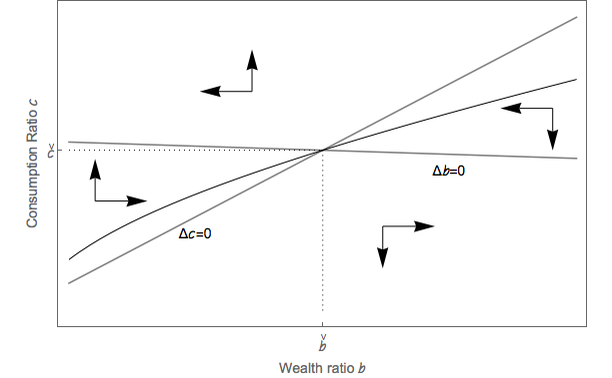
\includegraphics{./Figures/phaseDiag}
\caption{Phase Diagram}\label{fig:phaseDiag}
\end{figure}

We now determine the long-run target wealth-to-income ratio. Setting $\cRatE_{t+1}=\cRatE_t=\cTarg$ and $\cRatU_{t+1}=\MPC \bTarg$ in equation (\ref{eq:Explicit}) gives
\begin{equation}
\cTarg = \MPCU \left(1+\frac{\PatPGro^{-\CRRA}-1}{\urate}\right)^{1/\CRRA} \bTarg,
\label{eq:ssc}
\end{equation}
and setting $\bRatE_{t+1}=\bRatE_t=\bTarg$ and $\cRatE_t=\cTarg$ in equation (\ref{eq:ibcnorm}) gives,
\begin{equation}
\left(\PGro/\Rfree-1 \right) \bTarg = 1 -\cTarg. \label{eq:sss}
\end{equation}
Eliminating $\cTarg$ between (\ref{eq:ssc}) and (\ref{eq:sss}) then gives an explicit formula for the target wealth-to-income ratio,
\begin{verbatimwrite}{./Equations/bTargE}
\begin{equation}
 \bTarg= \left[\frac{\PGro}{\Rfree}-1+\MPCU \left(1+\frac{\PatPGro^{-\CRRA}-1}{\urate}\right)^{1/\CRRA}\right]^{-1}.
\label{eq:bTargE}
\end{equation}
\end{verbatimwrite}
\input ./Equations/bTargE.tex
Here is the intuition behind the target wealth ratio:  On the one hand,
consumers are growth-impatient, which prevents their wealth-to-income ratio
from heading off to infinity.  On the other hand, consumers have
a precautionary motive that intensifies more and more as the level of
wealth gets lower and lower.  At some point as wealth declines, the precautionary motive
gets strong enough to counterbalance impatience.  The point where impatience matches prudence defines the target wealth-to-income ratio.

Expression (\ref{eq:bTargE}) encapsulates several of the key economic
effects captured by the model.  The human wealth effect of growth is
captured by the $\PGro$ and $\PatPGro$ terms. Increasing $\PGro$ will
decrease the growth patience factor $\PatPGro$ and therefore reduce the
target level of wealth.  An increase in the worker's
patience (an increase in $\Discount$ and in the growth patience factor
$\PatPGro$) boosts the target level of wealth.  Finally, an increase in
unemployment risk increases the target level of precautionary wealth.\footnote{An increase in $\urate$ also decreases the worker's human wealth, because a greater probability of becoming unemployed means a greater risk of having zero income.  See \cite{ctDiscrete} for a careful analysis of the case of a human-wealth-preserving spread in risk.}
Those comparative statics results can be summarized as
\begin{eqnarray}
\frac{\partial \bTargE}{\partial \urate}   & > & 0, \label{eq:compstat}
\\ \frac{\partial \bTargE}{\partial \Discount} & >& 0, \nonumber
\\ \frac{\partial \bTargE}{\partial \PGro} & <& 0. \nonumber
\end{eqnarray}

The response of the target asset ratio to the risk aversion parameter
$\CRRA$ is less straightforward. On the one hand, higher risk aversion
enhances the demand for precautionary reserves. On the other hand, it
also implies that consumption is less elastic intertemporally.  The
response of $\bTargE$ to $\Rfree$ is also ambiguous, which is
unsurprising given that even in the deterministic model the relation
between interest rates and spending can be either positive or negative
depending on the relative sizes of the income, subsititution, and
human wealth effects.  In our model it is possible to show that if
$\CRRA \leq 1$, then the target level the wealth-to-income ratio
increases with the interest rate. For the usual case where $\CRRA >1$,
however, the sign of the response of $\bTargE$ to $\Rfree$ could be
positive or negative.


\subsection{Foreign Assets}

We now add up the individuals' balance sheets to find the country's
aggregate net foreign assets. We first present a general formula that
aggregates the resources of all generations of employed and unemployed
workers. We then specialize this formula under two assumptions about
the initial `stake' of newborns in the economy.  (A `stake' is a
transfer received by newborns). In the model without stakes, newborns
do not receive any transfer and must accumulate wealth through their
own frugality. Their microeconomic problem, therefore, is the one we
have described in the previous section. In the model with stakes,
newborns receive a transfer that puts their wealth-to-income ratio at
par with the rest of the population. The main advantage of the model
with stakes is that it is more tractable and yields a closed-form
expression for the ratio of net foreign assets to GDP.

\subsubsection{Aggregating Individual Wealths}

First, we focus on the wealth of the employed households. Calculations
in the appendix show that the ratio of employed workers' wealth to
output is given by
\begin{verbatimwrite}{./Equations/BRatEIndAgg}
\begin{eqnarray}
\BRatE_{t} = \frac{\BLevE_t}{\GDPLev_t} & = & (1-\kapShare) \left(1-\underbrace{\frac{\erate\XperGro}{\EmpGro}}_{\equiv \LGro}\right) \sum_{n=0}^{+\infty}\LGro^{n} \bRatE_{t,t-n}, \label{eq:LGro} \label{eq:BRatEIndAgg}
\end{eqnarray}
\end{verbatimwrite}
\input ./Equations/BRatEIndAgg.tex
where $\bRatE_{t,t-n}$ is the wealth-to-income ratio at $t$ of the workers born at $t-n$, and $\LGro$ is the factor by which the share of a generation in total labor supply shrinks every period. Equation \eqref{eq:BRatEIndAgg}, thus, says that the ratio of workers' wealth to output is the average of the individual wealth-to-labor-income ratios over the past generations, weighted by the share of each generation in total labor supply and by the share of labor income in total output $(1-\kapShare)$.

Second, consider the wealth of the unemployed households (managed by the Blanchardian life insurance company). The aggregate wealth of unemployed households satisfies the dynamic equation,
\begin{equation*}
\BLevU_{t+1}= \Rfree (\BLevU_{t} -\CLevU_t)+ \urate \BLevE_{t+1},
\end{equation*}
where the first term on the right-hand side reflects the accumulation of wealth by the previously-unemployed households, and the second term is the wealth of newly-unemployed households. The unemployed households consume a constant fraction of their wealth, $\CLevU_t= \MPCU \BLevU_{t}$, so that the equation above can be rewritten,
\begin{verbatimwrite}{./Equations/BLevUtp1}
\begin{equation}
\BLevU_{t+1}= \Rfree (1-\MPCU) \BLevU_{t}+ \urate \BLevE_{t+1}.
\label{eq:BLevUtp1}
\end{equation}
\end{verbatimwrite}
\input ./Equations/BLevUtp1.tex
This equation fully characterizes the dynamics of the unemployed households' wealth ratio for a given path for the employed workers' wealth ratio.

\hypertarget{BuOyLev}{}

Now we consider a steady state in which the wealth of the employed is a constant fraction of GDP, $\BRatE = \BLevE /\GDPLev$. Then equation (\ref{eq:BLevUtp1}) and $\GDPLev_{t+1}/\GDPLev_t=\EmpGro \WGro$  imply that the ratio of wealth to GDP is also constant for unemployed households,\footnote{This expression assumes $\EmpGro \WGro >\PLives(\Discount \Rfree )^{1/\CRRA}$. Otherwise $\BLevU_{t} / \GDPLev_t$ grows without bound.}
\begin{equation}
\frac{\BLevU}{\GDPLev}= \frac{\urate \EmpGro \WGro}{\EmpGro \WGro -\PLives(\Discount \Rfree )^{1/\CRRA}} \frac{\BLevE}{\GDPLev}.
\label{eq:BuOyLev}
\end{equation}



The ratio of net foreign assets to GDP is obtained by subtracting domestic capital from domestic wealth. Using (\ref{eq:KOyLev}), (\ref{eq:NFALev}), (\ref{eq:BuOyLev}), $\GDPLev_{t+1}/\GDPLev_t=\EmpGro \WGro$, and $\BLev_t=\BLevE_t+\BLevU_{t}$, the ratio of net foreign assets to GDP is given by
\begin{verbatimwrite}{./Equations/NFARat}
\begin{equation}
\frac{\NFALev}{\GDPLev}= \frac{\EmpGro \WGro}{\Rfree} \left( 1 + \frac{\urate \EmpGro \WGro}{\EmpGro \WGro -\PLives(\Discount \Rfree )^{1/\CRRA}} \right) \frac{\BLevE}{\GDPLev} -\EmpGro \WGro\left( \frac{\kapShare}{\Rfree-\DeprFac}\right).
\label{eq:NFARat}
\end{equation}
\end{verbatimwrite}
\input ./Equations/NFARat
This expression gives the country's ratio of net foreign assets to GDP in terms of the exogenous parameters and one endogenous variable, the ratio of employed workers' wealth to GDP, $\BLevE/\GDPLev$. We now present two ways of pinning down the value of this endogenous variable.


\subsubsection{No Stake}

The most natural assumption is that newborns enter the economy with zero wealth, and must save some of their income to ensure that they do not starve
if they become unemployed.
In this case, analysis must be performed using simulation methods, because households of different ages will have different ratios of wealth to income.  (With a concave and nonanalytical consumption function, analytical aggregation cannot be performed.)

In this version of the model, each individual is faced with exactly
the same problem as in section 2.2. We denote by $\bRatE(n)$ the level
of normalized wealth held at the beginning of period $n$ of the
individual's life in the problem of section 2.2. We assume that the
individual starts his life with zero wealth, $\bRatE(0)=0$. In other
words, $\bRatE(n)_{n=0,1,2,..}$ is the optimal time path of the
individual's wealth. Then we can replace $\bRatE_{t,t-n}$ by
$\bRatE(n)$ in equation (\ref{eq:BRatEIndAgg}),
\begin{verbatimwrite}{./Equations/BRatENostake}
\begin{eqnarray}
\BRatE = \frac{\BLevE}{\GDPLev} & = & (1-\kapShare) (1-\LGro)\sum_{n=0}^{+\infty}\LGro^{n} \bRatE(n).
\label{eq:BRatENostake}
\end{eqnarray}
\end{verbatimwrite}
\input ./Equations/BRatENostake
The ratio of workers' wealth to GDP is constant, and can be computed numerically based on the path $\bRatE(n)_{n=0,1,...}$. Note that this ratio is lower than $(1-\kapShare) \bTargE$, since it is a weighted average of $(1-\kapShare) \bRatE(n)$, which converge toward $(1-\kapShare) \bTargE$ from below.



\subsubsection{A `Stake' That Yields a Representative Agent}

We now consider a version of the model in which an exogenous
redistribution program guarantees that the behavior of employed
households can be understood by analyzing the actions of a
``representative employed agent.'' This will be achieved by the
introduction of lump-sum transfers that ensure that the newborn
individuals are endowed with the same wealth-to-income ratio that
older generations already hold. This is explicitly {\it not} an
inheritance, as we have assumed that individuals have no bequest
motive and newborns are unrelated to anyone in the existing
population.  Our motivation is largely to make the model more
tractable, rather than to represent an important feature of the real
world; hence, we perform simulations designed to show that the
characteristics of the model with no `stake' are qualitatively and
quantitatively similar to those of the more tractable model with a
carefully chosen `stake.'


The details of the model with stakes are given in the appendix. The transfer ensures that the workers have the same wealth-to-income ratio at all times. Thus one can replace $\bRatE_{t,t-n}$ by $\bRatE_t$ in equation (\ref{eq:BRatEIndAgg}), which gives,
\begin{equation}
\BRatE_{t} = \frac{\BLevE_t}{\GDPLev_t}= (1-\kapShare ) \bRatE_t,
\label{eq:BRatEStakest}
\end{equation}
where $\BRatE_t$ follows the same saddle-point dynamics as for a single agent (adjusted for the transfer).

\hypertarget{bTargEStakes}{}
In the long run (see the appendix), $\bRatE_t$ converges to
\begin{verbatimwrite}{./Equations/bTargEStakes}
\begin{equation}
 \bTargTarg = \left[\frac{\PGro}{\Rfree}-\frac{1}{2-\LGro}+\MPCU \left(1+\frac{\PatPGro^{-\CRRA}-1}{\urate}\right)^{1/\CRRA}\right]^{-1}
\label{eq:bTargEStakes}
\end{equation}
\end{verbatimwrite}
\input ./Equations/bTargEStakes.tex
so that (\ref{eq:bTargEStakes}) implies a closed-form expression for the ratio of workers' wealth to GDP,\hypertarget{BRatEStakes}{}
\begin{verbatimwrite}{./Equations/BRatEStakes}
\begin{eqnarray}
\BTargTarg = \frac{\BLevE}{\GDPLev} & = & (1-\kapShare ) \bTargTarg.
\label{eq:BRatEStakes}
\end{eqnarray}
\end{verbatimwrite}
\input ./Equations/BRatEStakes.tex
This expression can be plugged into equation (\ref{eq:NFARat}) to find the ratio of net foreign assets to GDP.

It is interesting to compare formula (\ref{eq:bTargEStakes}) with the
one that we obtained for an individual in the model without
stakes---equation (\ref{eq:bTargE}). Since $\LGro<1$ we have
$\bTargTarg < \bTarg$. Thus
equations (\ref{eq:bTargE}) and (\ref{eq:bTargEStakes}) both predict
that the ratio of wealth to GDP is lower than $(1-\kapShare)
\bTarg$, but in the new formula this comes from the
fact that the target wealth-to-income ratio is lowered by the tax,
rather than from the fact that the wealth-to-income ratio is lower for
younger workers.

We will show below that the model with stakes provides a good
approximation to the model with no stake.  But the model with stakes has
several advantages. First, the transition dynamics can be
characterized using equation (\ref{eq:BRatEStakes}). In the model
without stakes the transition dynamics involve an infinite state space
as the wealth-to-income ratio must be tracked separately for each
generation. Second, the model with stakes gives a closed-form
expression for the steady state ratio of foreign assets to GDP. This
makes it possible to study analytically how the ratio of foreign
assets to GDP depends on the exogenous parameters of the model. With
formula (\ref{eq:BRatENostake}), by contrast, such a study must rely
on numerical simulations.

\section{Calibration and Simulation}

\hypertarget{calibration}{}
\subsection{Benchmark Calibration and Sensitivity Analysis}

Our benchmark calibration is reported in Table 1. The value for the unemployment probability, $\urate$, implies that a newborn worker expects to be employed for 40 years. The value for the probability of death, $\PDies$, implies that the expected lifetime of a newly unemployed worker is 20 years.

\medskip

%\centerline{\bf Table 1}
\begin{table}
  \caption{Calibration of Parameters}\label{table:calibration}
\begin{center}
\begin{tabular}{|c|c|c|c|c|c|c|c|c|c|}
  \hline
  % after \\: \hline or \cline{col1-col2} \cline{col3-col4} ...
  $\kapShare$ & $\DeprFac$ & $\EmpGro$ & $\WGro$ & $\Rfree$ & $\Discount^{-1}$ & $\XperGro$ & $\urate$ & $\CRRA$ & $\PDies$ \\ \hline
  0.3 & 0.94 & 1.01 & 1.04 & 1.04 & 1.04 & 1.01 & 0.025 & 2 & 0.05 \\
  \hline
\multicolumn{10}{l}{\small Note: For a reminder of parameter definitions, see Appendix \ref{AppDef}} \\
\end{tabular}
\end{center}
\end{table}

The long-run levels of $\bRatE$ and $\cRatE$ are given by
$\bTarg=4.85$ and $\cTarg=0.95$. The time paths for $\bRatE_{t}$ and $\cRatE_{t}$
are shown in Figure 2. The convergence to the targets is relatively
rapid. The individual saves more than one third of his income on
average in the first ten years of his life, after which his
wealth-to-income ratio already exceeds two thirds of the target
level. The wealth-to-income ratio reaches 99 percent of the target
level after 40 years (the average duration of employment).

For the benchmark calibration we find: $\KLev/\GDPLev=3$, $\NFALev/\GDPLev=0.420$ in the model with no stakes, and $\NFALev/\GDPLev=0.719$ in the model with stakes. These levels have the right order of magnitude (in view of the fact that most countries have a ratio of foreign assets to GDP between minus and plus 100 percent of GDP, based on the database of \cite{lmf:mark2}).

Figure 3 shows the sensitivity of $\NFALev/\GDPLev$ to changes in $\CRRA$, $\urate$, $\WGro$ and $\Rfree$. The death probability $\PDies$ was adjusted so as to keep the total expected lifetime of an individual equal to sixty years, i.e.,
\begin{eqnarray*}
\urate^{-1}+\PDies^{-1}=60.
\end{eqnarray*}

First, we observe that the model with stakes gives results that are higher than the model without stakes, but generally provides a good approximation for the variation of the net foreign assets with respect to the main parameters.

The variation with respect to the growth rate and the unemployment probability confirm theoretical properties derived earlier. The foreign assets ratio decreases with $\WGro$, as predicted by (\ref{eq:compstat}). The ratio of foreign assets to GDP also increases with the unemployment probability.
The ratio of foreign assets to GDP is increasing with risk aversion $\CRRA$.
Finally, the foreign asset ratio is increasing with $\Rfree$, mainly because of the impact of higher interest rates in reducing the ratio of physical capital to output. The wealth-to-GDP ratio (not reported in Figure 3) is not very sensitive to $\Rfree$, which is consistent with the ambiguity of the model prediction if $\CRRA >1$.

\medskip

\begin{figure}
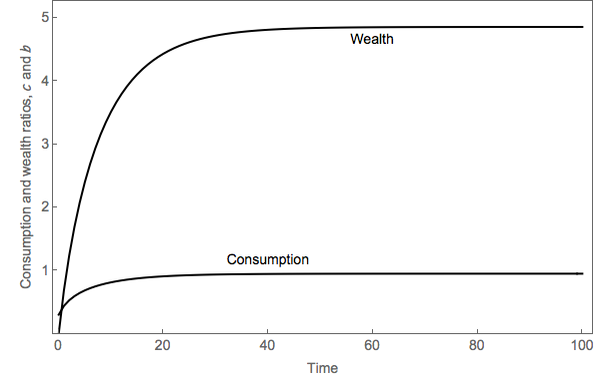
\includegraphics{./Figures/paths}
\caption{Transition Paths}\label{fig:paths}
\end{figure}

\medskip
\begin{figure}
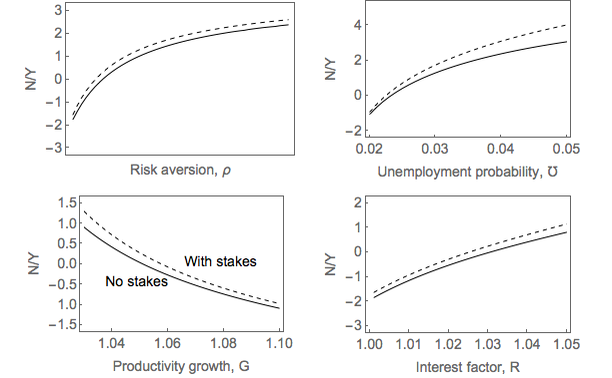
\includegraphics{./Figures/sensitivity}
\caption{Sensitivity To Parameters}\label{fig:sensitivity}
\end{figure}

\hypertarget{Translate-To-Realistic-Model}{}
\medskip
\subfile{./LaTeX/Insertions/Translate-To-Realistic-Model}
% \subsection{Robustness Check}

In this section, we show that the positive relationship between income uncertainty and the aggregate saving rate holds in a model with more realistic settings than the basic tractable model. Specifically, we use the model in \cite{cstwMPC} (henceforth 'CSTW'), which incorporates transitory and permanent shocks {\it a la} \cite{friedmanATheory} calibrated to match empirical estimates of such shocks in U.S.\ data.  We use this model to calculate a quantitative relationship between uncertainty and precautionary saving.

In the basic model, the only uncertainty comes from the shock of becoming unemployed. Here household income $y_{t}$ is determined by the aggregate wage rate $W_{t}$ and two idiosyncratic components, the permanent component $p_{t}$ and the transitory shock $\tshk_{t}$:
\begin{align}
y_{t}=p_{t}\tshk_{t}{W}_{t}
\end{align}
The permanent component follows:
\begin{align}
p_{t}=p_{t-1}\permShk_{t}
\end{align}
The transitory component is:
\begin{eqnarray}
  \xi_{t} & = & \mu \textrm{ with probability }\ \urate_{t}, \label{eq:tran}
\\ & = & (1-\tau_{t})\ell\theta_{t} \textrm{ with probability }\ 1-\urate_{t}, \nonumber
\end{eqnarray}
Here $\mu$ is the unemployment insurance payment when unemployed. $\tau_{t}$ is the rate of tax collected to pay unemployment benefits, $\ell$ is time worked per employee. $\permShk$ and $\theta$ are white noise drawn from log normal distribution and $\mathbb{E}_{t}\permShk_{t+n}=\mathbb{E}_{t}\theta_{t+n}=1\forall n>0$. By changing the value of $\sigma_{\permShk}$ and $\sigma_{\theta}$. we change the degree of uncertainty faced by households.The details of the model are described in appendix A.7

%In this model, the economy consists of a continuum of households of mass one distributed on the unit interval. Households die with a constant probability $D=1-\PLives$ between periods. This is different from the baseline model in which households only face probability of dying after they become unemployed. Each household maximize expected discount utility from consumption:
%\begin{eqnarray}
%\max\mathbb{E}_{t}\sum_{n=0}^{\infty}(\PLives\beta)^{n}\util(\cFunc_{t+n})
%\end{eqnarray}
%The household consumption functions satisfies:
%\begin{eqnarray}
%v(m_{t}) & = & \max_{c_{t}} \mathbb{E}_{t}\sum_{n=0}^{\infty}(\PLives\beta)^{n}\util(\cFunc_{t+n}), \label{eq:tran}
%\\ \text{s.t.}, \nonumber
%\\a_{t} & = & m_{t}-\c(m_{t})
%\\k_{t+1} & = & \frac{a_{t}}{\PLives \permShk_{t+1}}
%\\m_{t+1} & = & (\DeprFac+r_{t})k_{t+1}+\tshk_{t+1}
%\\a_{t} & \geq & 0
%\end{eqnarray}
%The production function is Cobb-Douglass:
%\begin{align}
%\end{align}
%The aggregate wage rate $W_{t}$ is determined by the aggregate productivity $Z_{t}$, capital stock $K_{t}$, and the aggregate supply of labor $L_{t}$:
%\begin{align}
%\end{align}
%$L_{t}$ is driven by two aggregate shocks:
%\begin{align}
%\\P_{t}=P_{t-1}\Psi_{t}
%\end{align}
%where $P_{t}$ is aggregate permanent productivity, 	$\Psi_{t}$ is the aggregate permanent shock
%and $\Theta_{t}$ is the aggregate transitory shock.\footnote{Note that $\Psi$ is the capitalized version of the Greek letter $\psi$ used for the idiosyncratic permanent shock; similarly $\Theta$ is the capitalized $\theta$}

The parameters are calibrated at the same level as they are in CSTW except for aggregate productivity growth rate and individual productivity growth rate. In CSTW, there is no aggregate and individual productivity growth; here we allow aggregate productivity growth $G=1.015$, and individual productivity growth $X=1.01$.

CSTW find that in order for the model to generate a plausible distribution of wealth it is necessary to build in some form of \textit{ex ante} hetergogeneity; we follow them in assuming that the time preference rate is the locus of heterogeneity. We calibrate the mean of the time discount factor to match the U.S.\ aggregate wealth to income ratio and the distribution of the time discount factor to match the wealth distribution among households in U.S.\ data.\footnote{The wealth to income ratio and wealth distribution data are obtained from the Survey of Consumer Finances.}

%\begin{eqnarray}
%a_{t} & = & m_{t}-\c(m_{t}), \label{eq:cons1}
%\\ k_{t+1}& = & \frac{a_{t}}{\pLive \permShk_{t+1}}, \label{eq:cons2}
%\end{eqnarray}

Following CSTW, we set the benchmark value of $\sigma_{\psi}^{2}$ and $\sigma_{\theta}^{2}$ to be $0.010\times4/11$ and $0.010\times4$. Under these new model settings, the growth impatience condition needs to be modified to be:

\begin{align}
	\PatPGroAdj = \frac{(\Discount \Rfree)^{1/\CRRA}\PLives}{\PGroAdj}
\end{align}
Where $\PGroAdj=\PGro \acute{\psi}$ and $\acute{\psi}\equiv (\mathbb{E}[\psi^{-1}])^{-1}$. By computing aggregate saving rate while increasing $\sigma_{\psi}^{2}$ and $\sigma_{\theta}^{2}$,  we derive the relationship between aggregate saving rate and the degree of uncertainty. Increasing $\sigma_{\psi}^{2}$ will also cause $\PGroAdj$ to increase. Agents with different $\beta$ have different $\PGroAdj$. The growth impatience condition $\PGroAdj<1$ of the most patient agent restricts the maximum value of $\sigma_{\psi}^{2}$ we can choose. Here we allow $\sigma_{\psi}^{2}$ and $\sigma_{\theta}^{2}$ to move from half of their benchmark values to twice the benchmark value.  Figure \ref{figure:savings} shows how the aggregate saving rate changes with $\sigma_{\psi}$. The first row in Table 2 reports the slope and $R^2$ calculated from OLS regression between the aggregate saving rate and the standard deviation of the permanent income shock. Under the model calibration, aggregate saving rate is almost perfectly correlated with the standard deviation of $\sigma_{\psi}$: adding 0.01 to $\sigma_{\psi}$ will cause the aggregate savings rate to rise about 0.83 percent. Figure \ref{figure:savingsTran} shows how the aggregate saving rate varies with the standard deviation of the transitory income shock. The regression result is reported in the second row of Table 2. The impact of transitory uncertainty is much smaller than the impact of permanent uncertainty. Increasing  $\sigma_{\theta}$ by 0.01 will cause the aggregate saving rate to increase by 0.011 percent. The last column reports the growth impatience factor of the most patient agent when $\sigma_{\psi}^{2}$ reaches its upper limit in each of the two exercises. We can see that the growth impatience condition is well satisfied in both exercises.
%\PatPGro
\begin{table}
	\centerline{\bf Table 2}
	\label{tab:Uncert}
	\begin{center}
		\begin{tabular}{ c c c c }
			\hline
			~ & Slope & $R^2$ & max $\PatPGro$\\
			\hline
			\multirow{2}{4em}{$\sigma_{\Psi}$} & 0.826 & \multirow{2}{*}{0.998} & \multirow{2}{4em}{0.998}\\
			& ($9.1\times10^{-3}$)***\\
			\multirow{2}{4em}{$\sigma_{\theta}$} & 0.0111 & \multirow{2}{*}{0.989} & \multirow{2}{4em}{0.996}\\
			& ($3.1\times10^{-4}$)***\\
			\hline
		\end{tabular}
		\\
	\end{center}
	\begin{tablenotes}
		\small
		\item Table 2 presents the correlation between the aggregate saving rate and the degree of income uncertainty. The first two columns show the slope and $R^2$ result from OLS regression. The third column show the growth impatience factor of the most patient agent in the economy. The first row shows the result of OLS regression between the aggregate saving rate and the standard deviation of permanent income shocks $\sigma_{\psi}$. The second row shows the result of OLS regression between the aggregate saving rate and the standard deviation of transitory income shocks $\sigma_{\theta}$. Standard errors are reported in parenthesis. ***represents significance level of 0.01.
	\end{tablenotes}
\end{table}

\begin{figure}[h]
	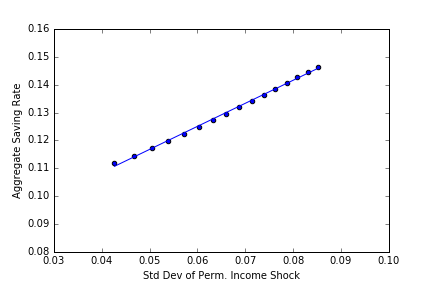
\includegraphics[scale=0.8]{\econtexRoot/LaTeX/Insertions/SavingVSPermShr_Youth_MPC_15.png}
	\centering
	\caption{Change in Savings Following increasing in Permanent Income Uncertainty}
	\label{figure:savings}

	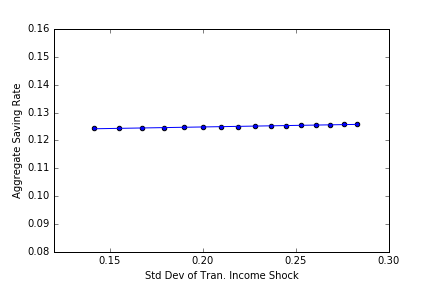
\includegraphics[scale=0.8]{\econtexRoot/LaTeX/Insertions/SavingVSTranShr_Youth_MPC_15.png}
	\centering
	\caption{Change in Savings Following increasing in Transitory Income Uncertainty}
	\label{figure:savingsTran}
\end{figure}



\subsection{Comparison with the Ramsey Model}

The Ramsey model corresponds to the particular case where the economy is populated by one representative infinitely-lived worker ($\EmpGro=1$ and $\urate=0$). Thus, one might expect our model to yield the same results as the Ramsey model in the limiting case as population growth and unemployment risk go to zero ($\PopGro$ and $\urate \rightarrow 0$).

In fact this is not the case. The predictions of our model for net foreign assets and capital flows exhibit a discontinuity at $\urate=0$. To see this, note that taking the limit of equation (\ref{eq:bTargE}) gives
\begin{equation*}
\lim_{\urate \rightarrow 0} \bTarg=0,
\end{equation*}
so that the ratio of total domestic wealth to GDP goes to zero as the risk of unemployment becomes vanishingly small,\footnote{This results from the fact that $\bRatE(n) \leq \bTargE$ converges to zero for all $n$. In the model with stakes this results from equation (\ref{eq:bTargEStakes}). }
\begin{equation*}
\lim_{\urate \rightarrow 0} \frac{\BLevE}{\GDPLev}=0,
\end{equation*}
implying that the ratio of foreign assets to GDP is equal to minus the ratio of capital to output,
\begin{equation}
\lim_{\urate \rightarrow 0} \frac{\NFALev}{\GDPLev}=-\frac{\KLev}{\GDPLev}.
\label{eq:NFARatIfUGt0}
\end{equation}

The Ramsey model does not yield the same formula. If the unemployment risk is strictly equal to zero ($\urate=0$), we must assume $\PGro < \Rfree$ for the intertemporal income of the worker to be well-defined and finite.\footnote{Note that this condition is not satisfied by the benchmark calibration in Table 1.} In this case income growth is the same at the individual level and at the aggregate level. We can also assume, without loss of generality, that $\XperGro=1$, so that $\PGro=\WGro$. Then it is possible to show that the asymptotic ratio of total net foreign assets to GDP is given by,
\begin{equation}
\lim_{t \rightarrow +\infty} \frac{\NFALev_t}{\GDPLev_t}=-\frac{\KLev}{\GDPLev}-\frac{1-\kapShare}{1-\WGro/\Rfree}
\label{eq:NFARatIfUEq0}
\end{equation}
(see the appendix).

Comparing (\ref{eq:NFARatIfUGt0}) with (\ref{eq:NFARatIfUEq0}) shows that the ratio of foreign assets to GDP is smaller in the Ramsey model. In fact, it is much smaller for plausible calibrations of the model. The ratio of gross foreign liabilities to GDP implied by the Ramsey model is close to 70 if $\Rfree =1.04$ and $\WGro =1.03$, and goes to infinity as $\WGro$ converges to $\Rfree$ from below. The growth impatience condition, which is necessary for the workers to have a finite target for their wealth to income ratio when they are vulnerable to unemployment, makes the infinitely-lived Ramsey consumer willing to borrow a lot against his future income.

The intuition for the discontinuity is that a consumer with CRRA
utility will never allow wealth to fall to zero if there is a
possibility of becoming permanently unemployed, because unemployment
with zero wealth yields an infinitely negative level of utility (if
$\CRRA>1$).  This is the reflection, in the international
macroeconomic context, of a result long understood in the
precautionary saving literature: Perfect foresight solutions are not
robust to the introduction of uninsurable noncapital income
shocks, even if those shocks occur with low probability.\footnote{Another interpretation is that the precautionary motive acts as a form of self-imposed liquidity constraint; see \cite{BufferStockTheory} for a formal proof of the equivalency, in the limit, of precautionary saving and liquidity constraints.}

\subsection{Social Insurance}

The model assumes that the income of an unemployed worker falls to
zero. This is a reasonable assumption for a country in which
unemployed and retired workers receive no social transfer (i.e., in
which there are no unemployment benefits and the retirement system is
entirely based on capitalization). However, many countries have such
transfers, and it is interesting to see their impact on foreign asset
accumulation in our model. We consider now the consequences if the
government creates a balanced-budget partial `unemployment insurance'
system.

Our definition of partial insurance starts by assuming that the `true'
labor income process is the one specified above, but the government
interferes with this process by transferring to the workers who become unemployed in period $t$ a multiple $\Severance$ of the labor income that they would have received if they had remained employed. The social insurance of our model could be interpreted as an unemployment benefit or as a pay-as-you-go retirement benefit.

The wealth of a newly-unemployed worker now includes the payment from the insurance scheme, so that equation (\ref{eq:cpfinfhorunemp}) becomes:
\begin{equation*}
\cLevU_{t}=\MPCU (\bLev^{u}_t+\Severance \Wage_t \labor_t)=\MPCU (\bRat^{u}_t+\Severance)\Wage_t \labor_t.
\end{equation*}
We introduce social insurance in the model with stakes.\footnote{Introducing social insurance in the model without stakes raises no conceptual problems, but does not yield a closed-form solution.} As shown in the appendix, one can compute the target wealth-to-GDP ratio as
\begin{verbatimwrite}{./Equations/bTargWithSocIns}
\begin{eqnarray}
\Alt{\bTarg}(\Severance) & = &
\left\{1-\Severance \left[\frac{\urate}{\EmpGro}+\MPCU \left(1+\frac{\PatPGro^{-\CRRA}-1}{\urate}\right)^{1/\CRRA}\right]\right\}\bTargTarg,
\label{eq:bTargWithSocIns}
\end{eqnarray}
\end{verbatimwrite}
\input ./Equations/bTargWithSocIns
where $\bTargTarg$ is the asset ratio without insurance, given by (\ref{eq:bTargEStakes}). The target wealth-to-income ratio is (linearly) decreasing with $\Severance$, as insurance provides a substitute to precautionary wealth. The formula for $\NFALev/\GDPLev$ remains (\ref{eq:NFARat}), with the ratio of workers' wealth to GDP given by,
\begin{equation}
\frac{\BLevE}{\GDPLev}=(1-\kapShare) \Alt{\bTarg}(\Severance).
\label{eq:STargWithSocIns}
\end{equation}
Figure 4 shows how the ratio of foreign assets to GDP, $\NFALev/\GDPLev$, varies with $\Severance$. The ratio decreases from 0.72 when there is no insurance to negative values when $\Severance$ exceeds 1 year of the worker's wage. The desired level of foreign assets is thus quite sensitive to the level of social insurance.

\medskip
\begin{figure}
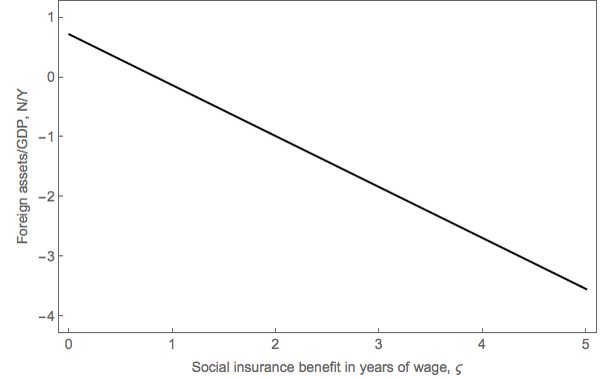
\includegraphics{./Figures/socIns}
\caption{Social Insurance Generosity and Net Foreign Assets}\label{fig:socIns}
\end{figure}

\medskip



\section{Applications}

Although the model is highly stylized, plausible calibrations can
predict ratios of foreign assets to GDP that are close to the levels
observed in the real world.\footnote{This fact obviously does not constitute a
test of the model (which would go beyond the scope of this paper), but
it suggests that the quantitative implications of the model cannot be
dismissed {\it prima facie} as irrelevant.} This section illustrates
how our framework can be applied by looking at two questions that have
been discussed in recent policy debates and academic research: The
relationship between economic development and capital flows, and the
long-run consequences of resorbing global imbalances.

\subsection{Economic Development and Capital Flows}

Many observers have noted the paradox that international flows of
capital have recently been going ``upstream'' from developing
countries (especially in Asia and most notably China) to the United
States. The case of China, which has caused so much consternation
recently, is merely the latest and largest example of a
long-established pattern: Over long time periods and in large samples
of developing countries, the countries that grow at a higher rate tend
to export more capital (see the evidence cited in footnote 1), a fact
that is difficult to reconcile with the standard neoclassical model of
growth (\cite{carroll&weil:crcs}; \cite{cow:habits};
\cite{gourinchasJeannePuzzle}; \cite{prs:brookings};
\cite{sandri:growthcapflows}). Can our model shed light on this
puzzle?

\subsubsection{Transitions}

In this section we look at the correlation between economic growth and
capital flows in a given country over time. We assume that the small
open economy enjoys an economic ``take-off,'' defined as a permanent
increase in the growth rate of productivity. However, the rate of
growth is not the only thing that increases at the time of the
transition: Idiosyncratic unemployment risk rises too. An increase in
idiosyncratic risk has been observed in many transition countries as
they adopt market systems, a development that has not been associated,
in most countries, with a corresponding increase in social
insurance. In particular, the rise in idiosyncratic risk has been
fingered as a reason for the very high saving rate in China (see,
e.g., \cite{cpChina} and the references therein).

Informally, we believe that our story also may relate to the
literature on rural-to-urban migration within developing countries.
That literature has long struggled to answer a simple question: Urban
wages are much higher than rural wages, so why doesn't everyone move
to the city?  Maybe the answer is ``cities are too risky.''  If, in
your home village, you are part of a well-developed and robust social
insurance network (based on extended family, clan, or village ties),
it might be perfectly rational to settle for a low but safe rural
standard of living in preference to the more lucrative, but also
riskier, life of a city dweller (under the presumption that moving
to the city would sever some or all of your ties to the village
network, and those ties could not quickly be replaced in a new
locale).  If people differ in their degree of risk tolerance, the
least risk averse will migrate to the cities, leaving the most
cautious behind; with a finite population, this could lead to equilibria
with large and permanent wage gaps.\footnote{See \cite{mrMobilityIndia} and
  work by \cite{townsendIndia} and coauthors.}

Formally, we assume that the economy starts from a steady state with
constant levels for the productivity growth rate and the unemployment
probability, $\WGro_b$ and $\urate_b$. At time $0$, those variables
unexpectedly jump to higher levels, $\WGro_a > \WGro_b$ and $\urate_a
> \urate_b$. The subscripts $b$ and $a$ respectively stand for
``before'' and ``after'' the transition. The death probability is
adjusted so as to keep the expected lifetime of an individual equal to
60 years.

Note that in order to benefit the domestic population, the transition must strictly increase the expected present value of an individual's labor income, given by
\begin{equation*}
\sum_{n=0}^{+\infty} \Rfree^{-n} \erate^{n} \labor_{t+n} \Wage_{t+n}= \frac{\Rfree}{\Rfree- \WGro \XperGro \erate} \labor_t \Wage_t.
\end{equation*}
Thus one must have,
\begin{equation}
\WGro_a \erate_a >\WGro_b \erate_b.
\label{eq:CondTransdyn}
\end{equation}
The increase in the idiosyncratic risk, in other words, should not be so large relative to the increase in the growth rate as to decrease workers' expected present value of labor income.

We consider the model with stakes, so that the transition dynamics for aggregate wealth can be derived from those for the representative agent. There is no social insurance. The appendix explains how the path of the main relevant variable can be computed. We are interested in whether capital tends to flow in or out of the country when the transition occurs.

For the sake of the simulation, we assume that the growth rate
increases from 2 percent to 6 percent in the transition, whereas the
unemployment probability increases from 2 percent to 3 percent
($\WGro_b=1.02$, $\urate_b=0.02$, and $\WGro_a=1.06$,
$\urate_a=0.03$). The other parameters remain calibrated as in Table
1.\footnote{With $\WGro=1.04$ and $\urate=0.025$, our benchmark
  calibration is the average of the pre-transition and post-transition
  regimes.} Note that condition (\ref{eq:CondTransdyn}) is satisfied:
indeed, the economic transition multiplies the expected present value
of individual labor income by a factor 20. If the risk of unemployment
did not increase with the transition, the expected net present value
of labor income would become infinite.

Figure~\ref{fig:transDyn} shows the time paths for the growth rate,
the ratio of net foreign assets to GDP and the ratio of capital
outflows to GDP, with and without the increase in unemployment
risk. Note that if unemployment risk increases, the growth rate takes
time to converge to its new higher level because the rate of labor
participation decreases over time, which dampens the acceleration of
growth. The figure also shows that the increase in idiosyncratic risk
has a large impact on the desired level of net foreign assets in the
long run---and thus on the direction of capital flows during the
transition. 

If the level of idiosyncratic risk remains the same, the
pickup in growth lowers the long-run level of foreign assets from
-23.9 percent to -135.6 percent of GDP, so that the higher growth rate
is associated with a larger volume of capital inflows, both in the
transition and in the long run. Thus, the model reproduces the usual
result from growth models without a precautionary motive: Higher expected growth
causes lower saving.

By contrast, if the level of idiosyncratic risk increases along with growth,
the long-run level of foreign assets increases to 69.7 percent of GDP,
implying that higher growth is associated with capital
outflows.\footnote{The pattern shown in figure 5 is robust to
  plausible changes in the values of the parameters. For example,
  higher growth remains associated with capital outflows if the
  post-transition growth rate is 8 percent instead of 6 percent
  (keeping $\urate_a$ equal to 3 percent) or if the unemployment
  probability increases to 2.5 percent instead of 3 percent (keeping
  the post-transition growth rate equal to 6 percent).} Thus, small
changes in the level of idiosyncratic risk have a first-order impact
on the volume and direction of capital flows and may help explain the
puzzling correlation between economic growth and capital flows that is
found in the data.\footnote{A similar point is made by
  \cite{sandri:growthcapflows}. In Sandri's model, the increase in the
  growth rate and in the level of idiosyncratic risk are jointly
  determined by the emergence of a class of entrepreneurs who invest
  in a risky technology, but must provide for the possibility of
  bankruptcy by putting aside riskless assets outside of their
  entrepreneurial activity.}

\medskip

\begin{figure}
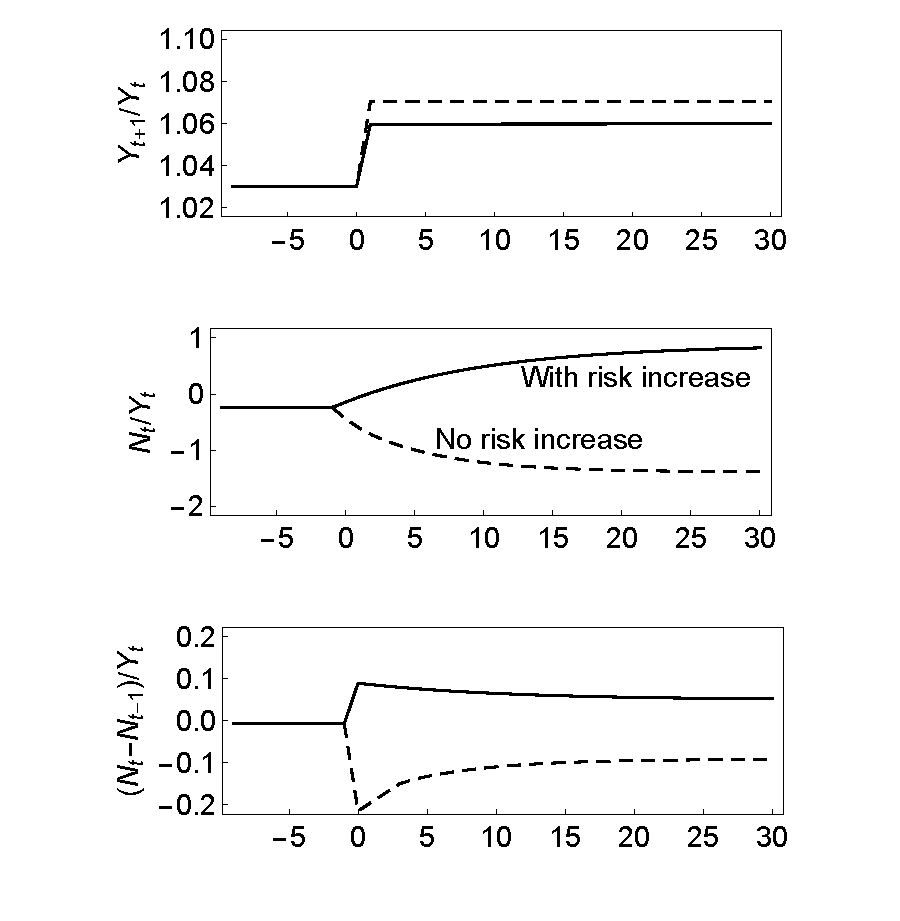
\includegraphics{./Figures/transDyn}
\caption{Transition Dynamics}\label{fig:transDyn}
\end{figure}
\medskip


\subsubsection{Steady States}

We now look at what the model says about the steady-state correlation between growth and capital flows, rather than the correlation for a given country over time. The country exports capital if its net foreign asset position is positive ($\NFALev>0$), since the level of its net foreign assets increases over time with output. The ratio of capital outflows to output is given by,
\begin{equation}
\frac{\NFALev_t-\NFALev_{t-1}}{\GDPLev_t}=\frac{\NFALev}{\GDPLev}\left(1 -\frac{1}{\EmpGro \WGro} \right).
\label{eq:DeltaFOyLev}
\end{equation}

On the one hand, with faster growth the target value of
$(\NFALev/\GDPLev)$ will be smaller.  On the other hand, a country
that grows faster must export more capital to maintain a constant
ratio of foreign assets to GDP (so the term in parentheses in
\eqref{eq:DeltaFOyLev} becomes larger).\footnote{See
  \cite{carroll:RiskyHabits} for further discussion of the possibility
  for precautionary models to generate a positive causality from
  growth to saving.}  Even if both initial and final values of
$(\NFALev/\GDPLev)$ are positive, the sign of the relation between
growth and net capital flows is theoretically ambiguous.

We calibrate the model with the pre-transition regime parameter values
(i.e.\ with $\WGro=1.02$ and $\urate=0.02$). Figure 6 shows how the
right-hand side of (\ref{eq:DeltaFOyLev}) varies with $\WGro$ under
two different assumptions. The line ``constant risk'' shows the ratio
of capital outflows to GDP if the only variable that changes is the
growth rate. The line ``increasing risk'' is based on the assumption
that the idiosyncratic risk increases linearly by 0.25 percent for
every additional percent of growth. Points A, B, and C respectively
correspond to the benchmark calibration, the pre-transition regime and
the post-transition regime of the previous section.

Two findings stand out. First, if idiosyncratic risk does not increase
with growth, the ratio of capital outflows to GDP is decreasing with
growth. Second, if idiosyncratic risk increases with growth as we have
specified, the ratio of capital outflows to output is positive, i.e.,
an increase in growth always causes the economy to export more capital
(even if it grows at 10 percent per year). The relationship between
the ratio of capital outflows to GDP and the growth rate is
non-monotonic. Capital outflows increase (as a share of GDP) with the
growth rate if the latter is lower than 6 percent. For higher levels
of the growth rate the sign of the relationship is reversed.

\medskip

\begin{figure}
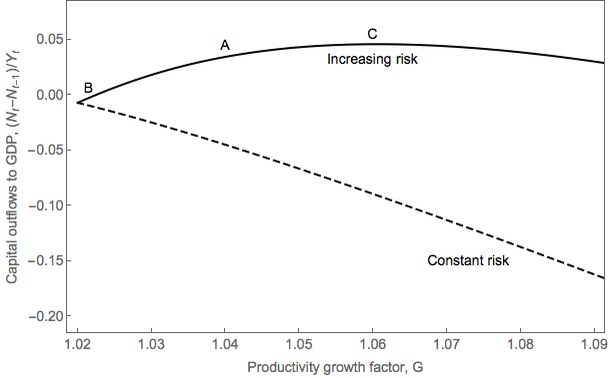
\includegraphics{./Figures/capOutflows}
\caption{Capital Outflows}\label{fig:capOutflows}
\end{figure}

\medskip


\subsection{Global Imbalances}

The main counterpart for the accumulation of net foreign assets by
developing countries has been the accumulation of net foreign
liabilities by the United States. In a famous 2005 speech, Ben
Bernanke hypothesized that the then-prevailing low level of world
interest rates and high level of U.S.\ current account deficits could
be due in part to this global ``savings glut''
(\cite{Bernanke:savingglut}). The U.S.\ authorities subsequently
argued that an orderly resolution of global financial imbalances
required the saving rate of Asian emerging market countries, most
notably China, to decrease to more normal levels.\footnote{The
    2008-09 global financial crisis added a further motivation for the
    same policy prescription: The maintenance of global aggregate
    demand.}

The small economy assumption is not appropriate for studying such
large events.  We therefore present in this section a two-country general
equilibrium version of the model that can be used instead. The model
is solved only for the steady state equilibria, which means that we
will be interested in the long-term consequences of particular policy
experiments. We first look at a closed-economy version of the model.

\subsubsection{Closed Economy}

We assume that the global economy has the same structure as the small
open economy that we have considered so far.  Global net foreign
assets are equal to zero, which using (\ref{eq:NFARat}) implies
\begin{equation}
\frac{1}{\Rfree} \left( 1 + \frac{\urate \EmpGro \WGro}{\EmpGro \WGro -\PLives(\Discount \Rfree )^{1/\CRRA}} \right) \frac{\BLevE}{\GDPLev} =\frac{\kapShare}{\Rfree-\DeprFac}.
\label{eq:closed}
\end{equation}
The left-hand side is the desired global stock of wealth whereas the
right-hand side is the desired global stock of capital. The equality
between the two endogenizes the steady-state interest rate. We assume
that the desired stock of wealth comes from the model with stakes and
social insurance, i.e., it is given by (\ref{eq:STargWithSocIns}).

Figure~\ref{fig:genEqbm} shows how the desired stocks of saving and of capital vary
with the interest rate for the benchmark calibration and three
different levels of social insurance $\Severance=0, 1$ and
$2$.\footnote{We would obtain similar results by varying parameters
  other than the level of social insurance. We choose social insurance
  (as opposed to, say, taste parameters such as the level of risk
  aversion) because it is a policy variable that can be changed.} The
desired level of capital is decreasing with the interest rate whereas
the desired level of wealth is increasing with the interest rate. Note
that the desired level of capital is much more sensitive to the
interest rate than the desired level of wealth. This implies that the
decrease in desired wealth generated by higher social insurance is
reflected almost one for one in a lower level of capital -- an interesting
point because it illustrates the importance of incorporating the precautionary
motive in the model.

\medskip

\begin{figure}
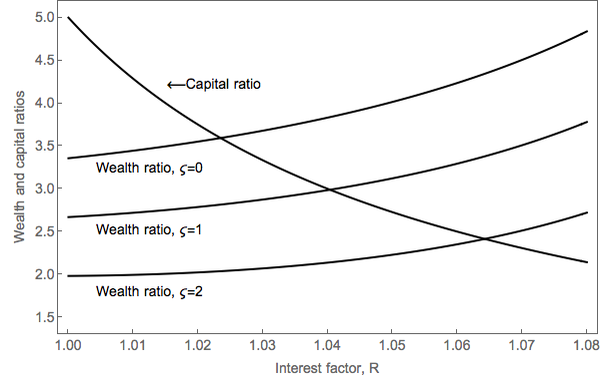
\includegraphics{./Figures/genEqbm}
\caption{General Equilibrium}\label{fig:genEqbm}
\end{figure}

\medskip

\subsubsection{Long-term Impact of Reducing Global Imbalances}

This section uses a two-country version of our model to investigate the long-run impact of a decrease in the desired stock of wealth outside of the United States. We consider a two-country world, where each country has the same structure as before. The two countries (denoted by $h$ and $f$, respectively for ``home'' and ``foreign'') are identical, except for their populations and levels of social insurance ($\Severance_h$ and $\Severance_f$). The shares of countries $h$ and $f$ in world output are respectively denoted by $\weight_h$ and $\weight_f$. The two countries have the same growth rate, so that there is a well-defined balanced growth path in which each country maintains a constant share of global output.

The condition that global foreign assets must be equal to zero,
\begin{equation*}
\NFALev_h+\NFALev_f=0,
\end{equation*}
endogenizes the global interest rate $\Rfree$. Normalizing by the countries' GDP, this equation can be rewritten,
\begin{equation*}
\weight_h \frac{\NFALev_h}{\GDPLev_h}+\weight_f \frac{\NFALev_f}{\GDPLev_f}=0,
\end{equation*}
where for each country, $\NFALev/\GDPLev$ is given by (\ref{eq:NFARat}), with $\BLevE/\GDPLev=(1-\kapShare)\Alt{\bTarg}(\Severance)$.

We consider the following experiment. Assume that the share of the
home country in total GDP is 20 percent ($\weight_h=0.2$ and
$\weight_f=0.8$), which is the right order of magnitude for the United
States. Assume that $\Severance_h > \Severance_f$, implying that the home
country has net liabilities because the desired ratio of wealth to GDP
is lower at home than in the rest of the world. We assume the values
$\Severance_h=1.5$ and $\Severance_f=0.75$, which implies $\Rfree=1.042$,
$\NFALev_h/\GDPLev_h=-0.512$ and $\NFALev_f/\GDPLev_f=0.128$ (the
values of the other parameters remaining as in Table 1). The ratio of
U.S.\ liabilities to GDP is higher than the current level (which is
closer to 25 percent), but not implausible looking forward if the
U.S.\ were to continue to maintain large current account deficits.

We then consider what would happen if global imbalances were resorbed
as a consequence of a reduction in the desired wealth-to-income ratio in the rest of the
world; this is achieved by increasing $\Severance_f$ to the home level (from 0.75 to
1.5). Figure 8 shows the long-run response of the foreign assets and
liabilities, as well as the global real interest rate and real wage
(normalized by productivity). As expected, the net foreign assets of
the home and foreign countries go to zero as the two countries
converge to the same ratio of wealth to GDP. However, this convergence
is achieved mainly by a decrease in global capital, which is reflected
in an increase in the real interest rate (from 4.2 to 5.6 percent),
and a decrease in the normalized real wage (by 5.4 percent).

The decrease in the desired foreign level of wealth thus has a large negative impact on the real wage. The welfare effect is unambiguously negative for the home country. The long-run welfare impact is also negative in the foreign country, although not necessarily during the transition, as the generations that are alive at the time of the increase in social insurance benefit from consuming the accumulated net foreign assets. The home country enjoys an export boom during the transition, but this is associated with lower investment rather than higher output.

The intuition should be clear from the analysis of the closed economy in the previous section. The decrease in the desired level of foreign wealth raises the world interest rate, with little impact on the level of home wealth. Thus, it is reflected mainly in a decrease in the ratio of capital to output, which depresses the real wage.

\medskip
\begin{figure}
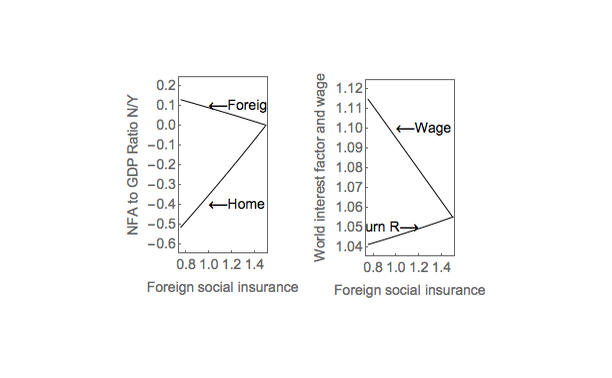
\includegraphics{./Figures/globImb}
\caption{Global Imbalances}\label{fig:globImb}
\end{figure}
\medskip

\section{Conclusion}

This paper has presented a tractable model of the net foreign assets
of a small open economy. The desired level of domestic wealth was
endogenized as the optimal level of precautionary wealth against an
idiosyncratic risk. We presented two applications of the model. The
first concerned the relationship between economic development and
capital flows.  The second concerned the long-run global implications
of reducing global imbalances by reducing the desired stock of saving
outside of the United States.

Although very stylized, the model is able to predict plausible orders
of magnitude for the ratio of net foreign assets to GDP. This being
said, there are several dimensions in which the model could be made
more realistic, at the expense of tractability. In
particular, it would be interesting to know the exchange rate
implications of a multi-goods extension of the model. (We anticipate
that such an extension would show that a developing country that
increases its desired level of foreign assets following economic
liberalization will see a depreciation of its real exchange rate.)  It
would be also interesting to look at the impact of changes in the
desired level of wealth on the price of assets other than currencies.

Our paper also has potential implications for future empirical
work. To the best of our knowledge, the empirical literature has not
looked at the impact of idiosyncratic risk and social insurance on net
foreign assets in the context of a large sample of countries. The available
evidence is anecdotal or focused on one country (e.g.,
\cite{cpChina}), or it is about financial development rather than
social insurance (\cite{mqrImbal}). It would be interesting to see if
the predictions of our framework for net foreign assets can be tested
with the available data (although we have not been able to find a cross-country
database on social insurance that could be used for such an empirical study).


\pagebreak\appendix
\setcounter{section}{0}
\setcounter{subsection}{0}

\section{Appendix}

\subsection{Key Model Parameters and Variables}
\label{AppDef}

We provide the following tables to aid the reader in keeping track of our notation.
\begin{center}
\begin{tabular}{|c|l|} \hline
 Parameter & \multicolumn{1}{|c|}{Definition}  \\ \hline
 $\kapShare$ & Capital's share in the Cobb-Douglas Production Function\\
 $\DeprFac$ & Depreciation Factor (Proportion Remaining After Depreciation)\\
 $\EmpGro$ & Population Growth Factor \\
 $\WGro$ & Aggregate Productivity Growth Factor\\
 $\Rfree$ & Riskfree Interest Factor \\
 $\Discount$ & Time Preference Factor \\
 $\CRRA$ & Coefficient of Relative Risk Aversion \\
 $\Severance$ & Severance Payment (In Years Of Income) Paid At Unemployment \\
 $\XperGro$ & Individual (eXperience-based) Productivity Growth \\
 $\weight_{i}$ & Weight (Share) Of Country $i$ in World Income \\
 $\urate$ & Probability Of Employed Worker Becoming Unemployed \\
 $\PDies $ & Probability of Death   \\
 $\Tax$ & Tax Rate \\
 $\xFer$ & `Stake' In Version Of Model With Stakes \\
 $\empState$ & Individual's Employment Status (1 if Employed; 0 if Not) \\
\hline
\end{tabular}
\end{center}

Some combinations of the parameters above are used as convenient shorthand:
\begin{center}
\begin{tabular}{|rcl|l|} \hline
 \multicolumn{3}{|c|}{Constant} & \multicolumn{1}{c|}{Definition}  \\ \hline
 $\erate$ & $\equiv$ & $1-\urate$ & Period Probability of Employed Worker Remaining Employed \\
 $\PLives$ & $\equiv$ & $1-\PDies$ & Probability of Survival (Not Dying) \\
 $\TaxFree$ & $\equiv$ & $1-\Tax$ & Proportion of Income Left After Taxation \\
 $\LGro$ & $\equiv$ & $\frac{\erate\XperGro}{\EmpGro}$ & Annual Shrinkage of Old Generations' Share in $\LLev$ \\
 $\MPCU$ & $\equiv$ & $1- \frac{(\Discount \Rfree)^{1/\CRRA}}{\Rfree/\PLives}$ & Marginal Propensity to Consume for Unemployed Consumer \\
 $\PGro$ & $\equiv$ & $\WGro \XperGro$ & Labor Income Growth For Continuing-Employed Individual \\
 $\PatPGro$ & $\equiv$ & $\frac{(\Discount \Rfree)^{1/\CRRA}}{\PGro}$ & Growth Patience Factor \\
\hline
\end{tabular}
\end{center}

\begin{center}
\begin{tabular}{|c|l|} \hline
 Variable & \multicolumn{1}{|c|}{Definition}  \\ \hline
 $\CRat$ & Consumption \\
 $\PopE$ & Employed Population \\
 $\IRat$ & Investment \\
 $\KRat$ & Physical Capital Stock \\
 $\LRat$ & Labor Supply \\
 $\labor$ & Individual labor productivity per employed worker \\
 $\NFARat$ & Net Foreign Assets \\
 $\GDPRat$ & GDP (`Production') \\
 $\BRat$ & Total Wealth (Foreign and Domestic) \\
 $\PopU$ & Unemployed Population \\
\hline
\end{tabular}
\end{center}

\begin{center}
\begin{tabular}{|c|l|} \hline
 Typeface & \multicolumn{1}{c|}{Meaning}  \\ \hline
 Bold & Level of a Variable \\
 Plain    & Ratio of The Variable To GDP or Labor Income  \\
 Uppercase & Aggregate Variable \\
 Lowercase    & Household-Level (Idiosyncratic) Variable  \\
\hline
\end{tabular}
\end{center}

\subsection{National Accounting}
\label{NatAc}

The aggregate budget constraint of residents can be written,
\begin{equation*}
\frac{\BLev_{t+1}}{\Rfree}+\CLev_t=\BLev_t+(1-\kapShare)\GDPLev_t.
\end{equation*}
Using (\ref{eq:MPK}) this equation can be rewritten as,
\begin{equation*}
\CLev_t+\ILev_t+\left(\NFALev_t-\Rfree \NFALev_{t-1} \right)=\GDPLev_t,
\end{equation*}
where $\ILev_t=\KLev_{t+1}- \DeprFac \KLev_t$ is domestic investment, and $\NFALev_t$ is given by (\ref{eq:NFALev}). Using the GDP identity (domestic output is either consumed, invested or exported),
and defining $\XLev$ as net exports, we have
\begin{equation*}
\CLev_t+\ILev_t+\XLev_t=\GDPLev_t,
\end{equation*}
it follows that net exports are equal to $\XLev_t=\NFALev_t-\Rfree \NFALev_{t-1}$. By definition, the current account balance is equal to net exports plus the income on net foreign assets,
\begin{equation*}
\text{Current Account}_t \equiv \XLev_t+\left(\Rfree-1 \right) \NFALev_{t-1},
\end{equation*}
from which we can derive the balance-of-payments equation,
\begin{equation*}
\text{Current Account}_t=\NFALev_t -\NFALev_{t-1}.
\end{equation*}
The current account balance is equal to the increase in the country's net foreign asset position, i.e., the volume of capital outflows in period $t$.

\subsection{The Consumption-Saving Problem of the Unemployed}

An insurance company {\it a la} \cite{blanchardFinite} provides each
newly unemployed worker with an annuity, i.e., a consumption path that
is conditional on the individual staying alive. The annuity contract
maximizes the welfare of the individual conditional on the expected
present value of his consumption being equal to his wealth. For a
worker becoming unemployed at $t$ it solves the problem,\footnote{Note that in a Blanchard model, the interest rate perceived by agents is \Rfree/\PLives~and the discount factor is \Discount \PLives.}
\begin{equation*}
 \max \sum_{n=0}^{+ \infty} \Discount^{n} \PLives^{n} \util(\cLev^u_{t+n})
\end{equation*}
subject to
\begin{eqnarray*}
\sum_{n=0}^{+ \infty} \Rfree^{-n} \PLives^{n} \cLev^u_{t+n} & = &\bLevU_t.
\end{eqnarray*}

The Euler equation is,
\begin{equation*}
\cLev_{t+n}^u=(\Discount \Rfree)^{n/\CRRA} \cLevU_{t}.
\end{equation*}
Using this expression to substitute out $\cLev^u_{t+n}$ from the expected present value constraint then gives,

\begin{equation*}
\bLevU_t = \sum_{n=0}^{+\infty} \Rfree^{-n} \PLives^{n} \cLev_{t+n}^u = \frac{\cLevU_{t}}{\MPCU}.
\end{equation*}

\subsection{Saddle-Point Stability}

We first characterize the iso-$\bRatE$ and iso-$\cRatE$ loci in the space $(\bRatE , \cRatE)$. Equation (\ref{eq:ibcnorm}) implies that the iso-$\bRatE$ locus is a line defined by,
\begin{equation*}
\cRatE = 1+\left(1-\frac{\PGro}{\Rfree} \right)\bRatE.
\end{equation*}

Similarly, setting $\cRatE_{t+1} = \cRatE_t$ in equation (\ref{eq:cetp1}) gives the following equation for the iso-$\cRatE$ locus,
\begin{equation*}
\cRatE = \left[1+\frac{\PGro}{\MPCU \Rfree}\left(1+\frac{\PatPGro^{-\CRRA}-1}{\urate}\right)^{-1/\CRRA}\right]^{-1} \left(1+ \bRatE \right).
\end{equation*}

The iso-$\cRatE$ locus is an upward-sloping line which intersects the $\cRatE$-axis below the iso-$\bRatE$ line. The iso-$\cRatE$ line and the iso-$\bRatE$ lines intersect in the positive quadrant (as indicated on Figure 1) if and only if $\bTarg > 0$. This is true because,

\begin{equation*}
\frac{\PGro}{\Rfree}-1+ \MPCU \left(1+\frac{\PatPGro^{-\CRRA}-1}{\urate}\right)^{1/\CRRA}
> \frac{\PGro}{\Rfree}-1+\MPCU = \frac{1}{\Rfree}\left(\PGro-(\Rfree \Discount)^{1/\CRRA}\right)>0,
\end{equation*}
where the last inequality follows from the growth impatience condition (\ref{eq:GIC}).

Using equation (\ref{eq:ibcnorm}), it is straightforward  to see that $\bRatE$ increases (decreases) if and only if $(\bRatE, \cRatE)$ is below (above) the iso-$\bRatE$ line. Equation (\ref{eq:cetp1}) implies that $\cRatE_{t+1}$ is decreasing with $\bRatE_t$. Therefore, $\cRatE$ decreases if and only if $(\bRatE, \cRatE)$ is in the region to the right of the iso-$\cRatE$ locus. This is also the region below the locus, because this locus is upward-sloping. Thus, the phase diagram is as it is shown on Figure 1, and the dynamics for the pair $(\bRatE _t, \cRatE_t)$ are saddle-point stable.


\subsection{Aggregating Individual Wealths}

Here we derive equation (\ref{eq:BRatEIndAgg}). The aggregate wealth of employed workers is given by,
\begin{equation*}
\BLevE_t=\sum_{n=0}^{+\infty} \popE_{t,t-n} \bLevE_{t,t-n}
\end{equation*}
where $\popE_{t,t-n}$ is the number of employed workers born in period $t-n$, and
$\bLevE_{t,t-n}=\bRatE_{t,t-n}\Wage_t \labor_{n}$ is the level of wealth held by the representative worker in the generation born at $t-n$. Using $\popE_{t,t-n}=\EmpGro^{t-n}\erate^{n}$ and $\labor_{n}=\XperGro^{n}\labor_0$ we have
\begin{equation*}
\BLevE_t = \EmpGro^t \labor_0 \Wage_t
\sum_{n=0}^{+\infty}\LGro^{n} \bRatE_{t,t-n},
\end{equation*}
with $\LGro = \erate \XperGro / \EmpGro$.
Using $\GDPLev_t=\Wage_t \LLev_t/(1-\kapShare)$ the ratio of foreign assets to output can be written
\begin{equation}
\frac{\BLevE_t}{\GDPLev_t}=(1-\kapShare) \frac{\EmpGro^t \labor_0} {\LLev_t} \sum_{n=0}^{+\infty}\LGro^{n} \bRatE_{t,t-n}.
\label{eq:BRatE}
\end{equation}
Each individual has a labor endowment that increases at rate $\XperGro$ until he becomes unemployed. Thus, in period $t$ the generation born at $t-n$ supplies a quantity of labor equal to the number of workers from this generation who are still employed at $t$, times the labor supply per worker,
\begin{eqnarray*}
\LLev_{t,t-n} & = & \EmpGro^{t-n}\erate^{n} \labor_0 \XperGro^{n}
= \EmpGro^{t} \LGro^{n}\labor_0 .
\end{eqnarray*}
Total labor supply, thus, is given by,
\begin{equation}
\LLev_t  =  \sum_{n=0}^{+\infty}\LLev_{t,t-n}  = \EmpGro^{t} \sum_{n=0}^{+\infty} \LGro^{n} \labor_0
=\EmpGro^{t} \frac{\labor_0}{1-\LGro}.
\label{eq:LLev}
\end{equation}
Using this expression to substitute out $\LLev_t$ from equation (\ref{eq:BRatE}) then gives equation  (\ref{eq:BRatEIndAgg}).

\subsection{Model with Stakes}

We add to the model a transfer that ensures that the workers have the same wealth-to-income ratio at all times. More precisely, the transfer ensures that if all workers have the same ratio $\bRatE$ in period $t$, then this is also true in period $t+1$. So one simply needs to assume that all workers had the same ratio $\bRatE$ at some point in the past for this to be true in all periods. This would be the case, for example, if the country started with a first generation at some distant period in the past.

The period-$t$ budget constraint of an individual is
\begin{equation*}
\frac{\bLev_{t+1}}{\Rfree}+ \cLev_{t}+\xFer_{t}=\bLev_{t}+\empState_{t} \labor_{t} \Wage_t,
\label{eq:ibcStakes}
\end{equation*}
where $\xFer_{t}$ is a lump-sum transfer. The transfer puts newborn individuals at the same net wealth-to-income ratio as the rest of the population. For the other workers the transfer is a lump-sum tax that is proportional to their generation's wealth. For an employed worker born at $t-n$ the tax is,
\begin{equation}
\xFer_{t}=\Tax \bRatE_t \labor_0 \XperGro^{n} \Wage_t, \label{eq:xFerE}
\end{equation}
whereas for a new-born worker the transfer is given by,
\begin{equation}
\xFer_{t}=-\overbrace{\TaxFree}^{\equiv 1-\Tax} \bRatE_t \labor_0 \Wage_t. \label{eq:xFerAtBirth}
\end{equation}

In all periods of a worker's life, thus, the normalized budget constraint is given by,
\begin{verbatimwrite}{./Equations/ibcnormStakes}
\begin{equation}
\bRatE_{t+1} = (\Rfree /\PGro) \left(\TaxFree \bRatE_{t} -\cRatE_{t}+1\right),
\label{eq:ibcnormStakes}
\end{equation}
\end{verbatimwrite}
\input ./Equations/ibcnormStakes
which generalizes (\ref{eq:ibcnorm}). Equation (\ref{eq:ssc}) remains valid,
\begin{equation*}
\cTargTarg = \MPCU \left(1+\frac{\PatPGro^{-\CRRA}-1}{\urate}\right)^{1/\CRRA} \bTargTarg,
\end{equation*}
whereas (\ref{eq:sss}) is replaced by
\begin{equation*}
\left(\PGro/\Rfree-\TaxFree \right) \bTargTarg = 1 -\cTargTarg.
\end{equation*}
Eliminating $\cTargTarg$ between these two equations then gives the following expression for the target wealth-to-income ratio,
\begin{equation}
 \bTargTarg= \left[\frac{\PGro}{\Rfree}-\TaxFree+\MPCU \left(1+\frac{\PatPGro^{-\CRRA}-1}{\urate}\right)^{1/\CRRA}\right]^{-1}.
\label{eq:bTargE_tau}
\end{equation}
The equilibrium level of $\Tax$ results from the following equality,
\begin{equation*}
\EmpGro^t \TaxFree \bRatE_t \labor_0 \Wage_t  = \Tax \bRatE_t \Wage_t \LLev_t.
\label{eq:gbc}
\end{equation*}
The left-hand side is the flow of payment that is required to endow each newborn individual with the same ratio of after-tax net wealth to income as the rest of the population. The right-hand side is the proceeds of the tax on the employed workers. Using (\ref{eq:LLev}) to substitute out $\LLev_t$, this equation simplifies to $\TaxFree = \Tax / (1-
\LGro)$, which implies
\begin{equation}
\Tax=\frac{1-\LGro}{2-\LGro}.
\label{eq:tau}
\end{equation}
Using this expression to substitute out $\Tax$ from (\ref{eq:bTargE_tau}) gives (\ref{eq:bTargEStakes}).

\medskip
% \subsection{Model with Time Preference Heterogeneity}

In this model, the economy consists of a continuum of households of mass one distributed on the unit interval. Households die with a constant probability $D=1-\PLives$ between periods. This is different from the baseline model in which households only face probability of dying after they become unemployed. The income process of a household has been described in section 3.2. Each household maximizes expected discount utility from consumption:
\begin{eqnarray}
\max\mathbb{E}_{t}\sum_{n=0}^{\infty}(\PLives\beta)^{n}\util(\cFunc_{t+n})
\end{eqnarray}
The household consumption functions satisfies:
\begin{eqnarray}
v(m_{t}) & = & \max_{c_{t}} \util(\cFunc_{t}(m_{t}))+\beta\PLives\mathbb{E}_{t}(\permShk_{t+1})^{1-\rho}v(m_{t+1}), \label{eq:tran}
\\ \text{s.t.}, \nonumber
\\a_{t} & = & m_{t}-\cFunc(m_{t})
\\k_{t+1} & = & \frac{a_{t}}{\PLives \permShk_{t+1}}
\\m_{t+1} & = & (\DeprFac+r_{t})k_{t+1}+\tshk_{t+1}
\\a_{t} & \geq & 0
\end{eqnarray}
where the variables are divided by the level of permanent income $\pLev = p_{t}\pmb{W}$, so that
when aggregate shocks are shut down, the only state variable is (normalized) cash-on hand $m_{t}$.
The production function is Cobb-Douglass:
\begin{align}
ZK^{\alpha}(\ell L)^{1-\alpha}
\end{align}
The aggregate wage rate $\pmb{W}_{t}$ is determined by the aggregate productivity $Z_{t}$, capital stock $K_{t}$, and the aggregate supply of labor $L_{t}$:
\begin{align}
\pmb{W}_{t}=(1-\alpha)Z_{t}(\frac{K_{t}}{\ell L})^{\alpha}
\end{align}
$L_{t}$ is driven by two aggregate shocks:
\begin{align}
L_{t}=P_{t}\Theta_{t}
\\P_{t}=P_{t-1}\Psi_{t}
\end{align}
where $P_{t}$ is aggregate permanent productivity, 	$\Psi_{t}$ is the aggregate permanent shock
and $\Theta_{t}$ is the aggregate transitory shock.\footnote{Note that $\Psi$ is the capitalized version of the Greek letter $\psi$ used for the idiosyncratic permanent shock; similarly $\Theta$ is the capitalized $\theta$}


\subfile{./LaTeX/Insertions/Translate-To-Realistic-Model-Appendix}
\subsection{The Ramsey Model}

The Ramsey model corresponds to the particular case where there is one representative infinitely-lived worker ($\EmpGro=1$ and $\urate=0$). In this case income growth is the same at the individual level and at the aggregate level. We can assume, without loss of generality, that $\XperGro=1$, so that $\PGro=\WGro$.

The individual's problem at time $0$ is to maximize,
\begin{equation*}
\sum_{t=0}^{+\infty} \Discount^t \util(\cLev_t),
\end{equation*}
subject to the budget constraint,
\begin{equation*}
\frac{\bLev_{t+1}}{\Rfree}+\cLev_t=\bLev_t+ (1-\kapShare) \gdpLev_t,
\end{equation*}
where $\gdpLev_t=\WGro^t \gdpLev_0$ is the country's output. For the worker's discounted intertemporal income to be finite we must assume $\WGro <\Rfree$.

Iterating on the budget constraint and using $\cLev_t=(\Discount \Rfree )^{t/\CRRA} \cLev_0$ (from the Euler equation) and $\gdpLev_t=\WGro^t \gdpLev_0$ to substitute out consumption and output, we have
\begin{eqnarray*}
\bLev_t&=&\sum_{n=0}^{t-1}\Rfree^{t-n} (1-\kapShare) \gdpLev_n - \sum_{n=0}^{t-1}\Rfree^{t-n} \cLev_n+\Rfree^t \bLev_0,
\\ &=& (1-\kapShare) \gdpLev_0 \frac{\Rfree^t -\WGro^t}{1-\WGro/\Rfree}-\cLev_0 \frac{\Rfree^t -(\Discount \Rfree )^{t/\CRRA}}{1-(\Discount \Rfree )^{1/\CRRA}/\Rfree}+\Rfree^t \bLev_0.
\end{eqnarray*}
For the transversality condition to be satisfied, $\cLev_0$ must be such that the terms in $\Rfree^t$ cancel out in the expression above. Using this property to substitute out $\cLev_0$, the expression for $\bLev_t$ simplifies to,
\begin{equation*}
\bLev_t = (1-\kapShare) \gdpLev_0 \frac{(\Discount \Rfree )^{t/\CRRA}-\WGro^t}{1-\WGro/\Rfree} +\bLev_0 (\Discount \Rfree )^{t/\CRRA}.
\end{equation*}
The limiting wealth-to-output ratio is given by,
\begin{eqnarray*}
\lim_{t \rightarrow +\infty} \frac{\bLev_t}{\gdpLev_t}&=& \lim_{t \rightarrow +\infty}
\frac{1-\kapShare}{\WGro^{t}} \frac{(\Discount \Rfree )^{t/\CRRA}-\WGro^t}{1-\WGro/\Rfree}
+\frac{\bLev_0}{\gdpLev_0}\frac{(\Discount \Rfree )^{t/\CRRA}}{\WGro^t},  \\
 &=& \lim_{t \rightarrow +\infty}(1-\kapShare) \frac{\PatPGro^t-1}{1-\WGro/\Rfree}+\frac{\bLev_0}{\gdpLev_0}\PatPGro^t  \\
 &=& -\frac{1-\kapShare}{1-\WGro/\Rfree}.
 \end{eqnarray*}

\subsection{Social Insurance}

Here we derive equation (\ref{eq:bTargWithSocIns}). The worker's normalized budget constraint is still given by (\ref{eq:ibcnormStakes}), taking into account that the wage is taxed at rate $\Tax_w$ to pay for the unemployment benefits,
\begin{equation}
\bRatE_{t+1} = (\Rfree/\PGro)\left(\TaxFree \bRatE_{t} -\cRatE_{t}+\TaxFree_w\right).
\label{eq:ibcnormStakesSocins}
\end{equation}
Equation (\ref{eq:Explicit}) still applies, with $\cRatU_{t+1}=\MPCU (\bRatE_{t+1}+\Severance)$. Setting $\bRatE_{t+1}=\bRatE_t=\Alt{\bTarg}$ and $\cRatE_{t+1}=\cRatE_t=\Alt{\cTarg}$ in equations (\ref{eq:Explicit}) and (\ref{eq:ibcnormStakesSocins}) we obtain
\begin{eqnarray*}
\Alt{\cTarg}= \MPCU \left(1+\frac{\PatPGro^{-1/\CRRA}-1}{\urate}\right)^{1/\CRRA}  (\Alt{\bTarg}+\Severance),
\end{eqnarray*}
\begin{eqnarray*}
\Alt{\bTarg} \left( \PGro /\Rfree -\TaxFree \right) = \TaxFree_w - \Alt{\cTarg}.
\end{eqnarray*}
Eliminating $\Alt{\cTarg}$ between these equations gives,
\begin{equation}
\Alt{\bTarg} = \left[ \TaxFree_w - \MPCU \left(1+\frac{\PatPGro^{-\CRRA}-1}{\urate}\right)^{1/\CRRA} \Severance \right] \bTargTarg,
\label{eq:stargsi}
\end{equation}
where $\bTargTarg$ is given by equation (\ref{eq:bTargEStakes}).
The tax rate $\Tax_w$ must satisfy
\begin{equation}
\Tax_w \LLev_t \Wage_t =\urate \PopE_{t-1} \labor_{t} \Severance \Wage_t. \label{eq:taxBalance}
\end{equation}
The left-hand-side is the flow of tax receipts at time $t$. The right-hand-side is the amount needed to finance the transfer to the newly unemployed workers. Using $\labor_{t}=\LLev_t /\PopE_t$ and $\PopE_t / \PopE_{t-1}= \EmpGro$ one has,
\begin{equation*}
\Tax_w = \frac{\urate}{\EmpGro} \Severance.
\end{equation*}
Using this expression and (\ref{eq:tau}) to substitute out $\Tax_w$ from equation (\ref{eq:stargsi}) gives equation (\ref{eq:bTargWithSocIns}).

\subsection{Transition Dynamics}

Normalizing $\labor_0$ to 1, the equation for the dynamics of aggregate labor supply is,
\begin{equation*}
\LLev_t=\erate \XperGro \LLev_{t-1}+\EmpGro^t,
\end{equation*}
implying that in steady state,
\begin{equation*}
\LLev_t = \frac{\EmpGro^{t+1}}{\EmpGro-\erate \XperGro}.
\end{equation*}
Up until period $0$ (inclusive), the economy is in a steady growth path with $\WGro=\WGro_b$ and $\urate=\urate_b$, so that
\begin{equation*}
\LLev_0=\frac{\EmpGro}{\EmpGro-\erate_b \XperGro}.
\end{equation*}
In period $0$ it is announced that from period $1$ onwards the productivity growth rate and the flow probability of unemployment jump to higher levels, $\WGro_a$ and $\urate_a$. Starting from $\LLev_0$, the dynamics of labor supply are given by,
\begin{equation*}
\LLev_t=\erate_a \XperGro \LLev_{t-1}+\EmpGro^t,
\end{equation*}
from which it is possible to compute the whole path $(\LLev_t)_{t\leq0}$, as well as the gross rate of growth in labor supply, $\LLev_t/\LLev_{t-1}$. It follows from (\ref{eq:Cobb-Douglas}) and (\ref{eq:MPK}) that output grows at the same rate as $z_t \LLev_t$. Hence the gross rate of output growth, $\GDPGro_{t} \equiv \GDPLev_t/\GDPLev_{t-1}$, is given by
\begin{equation*}
\GDPGro_{t}=\WGro_a \LLev_t/\LLev_{t-1}
\end{equation*}
for $t \geq 1$. Using this expression we can compute the whole path $(\GDPGro_{t})_{t \geq 1}$.

We now come to the ratios of net foreign assets and capital outflows to GDP, $\NFALev_t/\GDPLev_t$ and $(\NFALev_t -\NFALev_{t-1})/\GDPLev_t$. Using the definition of $\NFALev$ equation (\ref{eq:NFALev}), we have
\begin{equation*}
\frac{\NFALev_t}{\GDPLev_t}=\GDPGro_{t+1} \left[ \frac{(1-\kapShare) \bRat_{t+1}}{\Rfree} -\frac{\KLev}{\GDPLev} \right],
\end{equation*}
\begin{equation*}
\frac{\NFALev_t -\NFALev_{t-1}}{\GDPLev_t}=\frac{1-\kapShare}{\Rfree} \left( \GDPGro_{t+1} \bRat_{t+1} -\bRat_t \right) -(\GDPGro_{t+1}-1)\frac{\KLev}{\GDPLev},
\end{equation*}
where $\bRat_t=\bRatE_t+\bRatU_t$ is the ratio of aggregate wealth to aggregate labor income. The path for $\bRatE_t$ is the individual convergence path for the model with stakes, where the initial condition $\bRatE_0$ is given by (\ref{eq:bTargEStakes}) with $\WGro = \WGro_b$ and $\urate = \urate_b$. This gives us the whole path $(\bRatE_t)_{t \leq 0}$.
As for $\bRatU_t$, the initial condition can be derived from equation (\ref{eq:BuOyLev}),
\begin{equation*}
\bRatU_0= \frac{\urate_b \EmpGro \WGro_b}{\EmpGro \WGro_b -\PLives_b(\Discount \Rfree )^{1/\CRRA}} \bRatE_0.
\end{equation*}
The path for $\bRatU_t$ can then be derived from equation
(\ref{eq:BLevUtp1}), which can be rewritten in normalized form,
\begin{verbatimwrite}{./Equations/bRatUtp1}
\begin{equation*}
\bRatU_{t+1}=\frac{\PLives_a(\Discount \Rfree)^{1/\CRRA}}{\GDPGro_{t+1}} \bRatU_t + \urate_a \bRatE_{t+1}.
\end{equation*}
\end{verbatimwrite}
\input ./Equations/bRatUtp1

\subsection{Consumption Function}

Here we describe our algorithm for finding the consumption
function.

We know two points on the ``true'' consumption function: For wealth of
zero, consumption must be zero; and for wealth equal to its target value,
consumption must equal its target value.  We can thus construct a crude starting approximation
to the consumption function as $_0\cFunc^{e}(\bRatE) = (\cTarg/\bTarg)\bRatE$,
the unique line that goes through the points $\{0.,0.\}$ and $\{\bTarg,\cTarg\}$ (where
the 0 presubscript indicates that we have executed zero iterations of the `improvement' algorithm
described below).

We will need to improve upon this approximation considerably in order
to obtain a satisfactory solution to the model.  Our first step is to
construct a set of points at which to evaluate any approximating function, which
we choose on the interval $[0,2\bTarg]$. Dividing that interval equally into $n$ subintervals, we
obtain a set of states $\bRat[i]=2 \bTarg (i/n)$ for $i=0,1,...,n$.

Now rewrite the Euler equation \eqref{eq:Explicit} as
\begin{equation*}
    \cRatE_t= \frac{1}{\PatPGro }\left( \erate (\cFunc^{e}_{t+1})^{-\CRRA}+\urate (\cRatU_{t+1})^{-\CRRA} \right)^{-1/\CRRA}
\end{equation*}
and note that starting with iteration $m=0$ we can generate a `next' set of consumption points from the current points using
\begin{equation}
    _{m+1}\cRatE[i]= \frac{1}{\PatPGro }\left( \erate (_{m}\cFunc^{e}((\Rfree/\PGro)\left(\bRatE[i] -_{m}\cRatE[i]+1\right))^{-\CRRA}+\urate (\MPCU (\Rfree/\PGro)\left(\bRatE[i] -_{m}\cRatE[i]+1\right))^{-\CRRA} \right)^{-1/\CRRA}
\label{eq:EulerMod}
\end{equation}

We solve by using iteration. The iterative scheme stops when
successive approximate consumption functions change little at grids.

Given the initial function for $m=0$, $_{0}\cFunc^{e}(\bRat)$, the algorithm can be summarized as follows:
\begin{enumerate}
  \item Compute the points $_{m+1}\cRatE[i]$ using \eqref{eq:EulerMod}
  \item Construct an approximate function $_{m+1}\cFunc^{e}(\bRat)$ by fitting the points $(\bRat[i],_{m+1}\cRatE[i])$
  \item If $\max|_{m+1}\cRatE[i]-_{m}\cRatE[i]|<\epsilon$, stop; else increment $m$ and go to step 1
  \end{enumerate}

  
\newpage

\bibliography{\texname,\texname-Add,economics}

\end{document}

